\documentclass[10pt]{article}

% amsmath package, useful for mathematical formulas
\usepackage{amsmath}
% amssymb package, useful for mathematical symbols
\usepackage{amssymb}

% graphicx package, useful for including eps and pdf graphics
% include graphics with the command \includegraphics
\usepackage{graphicx}

% cite package, to clean up citations in the main text. Do not remove.
\usepackage{cite}

\usepackage{color} 

% Use doublespacing - comment out for single spacing
%\usepackage{setspace} 
%\doublespacing


% Text layout
\topmargin 0.0cm
\oddsidemargin 0.5cm
\evensidemargin 0.5cm
\textwidth 16cm 
\textheight 21cm

% Bold the 'Figure #' in the caption and separate it with a period
% Captions will be left justified
\usepackage[labelfont=bf,labelsep=period,justification=raggedright]{caption}

% Use the PLoS provided bibtex style
\bibliographystyle{PLoS2009}

% Remove brackets from numbering in List of References
\makeatletter
\renewcommand{\@biblabel}[1]{\quad#1.}
\makeatother


% Leave date blank
\date{}

\pagestyle{myheadings}
%% ** EDIT HERE **
%% Please insert a running head of 30 characters or less.  
%% Include it twice, once between each set of braces
\markboth{Evolutionary modeling}{Evolutionary modeling}

%% ** EDIT HERE **
%% PLEASE INCLUDE ALL MACROS BELOW
\usepackage{setspace}
\doublespacing

%parsetree.sty - LaTeX style file with macros for typesetting parse trees
% See parsetree.doc for extensive section-by-section comments to the code.
% Eirik Hektoen, 1994-2-24

\typeout{Including style file `parsetree.sty'.}


% Some Initial Variables and Auxiliary Macros:

\def\pterror#1{\errmessage{Parsetree ERROR: #1}}

\newdimen\pthgap\def\pthorgap#1{\pthgap=#1}
\newdimen\ptvgap\def\ptvergap#1{\ptvgap=#1}

\newbox\ptnodestrutbox\def\ptnodestrut{\unhcopy\ptnodestrutbox}
\newbox\ptleafstrutbox\def\ptleafstrut{\unhcopy\ptleafstrutbox}

\def\ptnodefont#1#2#3{\def\ptnodefn{#1}
  \setbox\ptnodestrutbox=\hbox{\vrule height#2 width0pt depth#3}}
\def\ptleaffont#1#2#3{\def\ptleaffn{#1}
  \setbox\ptleafstrutbox=\hbox{\vrule height#2 width0pt depth#3}}


% Customizable Definitions (- NOTE: MAY BE REDEFINED IN DOCUMENT -):

\pthorgap{12pt}                         % horizontal gap betw sisters
\ptvergap{12pt}                         % vertical gap betw mother/daughter
\ptnodefont{\normalsize\rm}{11pt}{3pt}  % font and strut height/depth: nodes
\ptleaffont{\normalsize\it}{11pt}{3pt}  % font and strut height/depth: leaves


% Hierarchy-building macros:

\newcount\ptdepth           % current bracketing depth
\newcount\ptn               % 1: m, 2: ma, 3: mab, 4: mabc
\newbox\ptm \newdimen\ptmx  % m = mother
\newbox\pta \newdimen\ptax  % a = 1st daughter
\newbox\ptb \newdimen\ptbx  % b = 2nd daughter
\newbox\ptc \newdimen\ptcx  % c = 3rd daughter (max)
\newbox\ptx \newdimen\ptxx  % x = used for passing results
\newif\ifpttri              % choose triangular subtree with \pttritrue

\def\ptnext{\advance\ptn by 1 \ifcase\ptn
  \or \setbox\ptm=\box\ptx \ptmx=\ptxx \or \setbox\pta=\box\ptx \ptax=\ptxx
  \or \setbox\ptb=\box\ptx \ptbx=\ptxx \or \setbox\ptc=\box\ptx \ptcx=\ptxx
  \else \pterror{More than 3 daughters in (sub)tree}\fi}

\def\ptbegtree{\ptdepth=0}
\def\ptendtree
  {\ifnum\ptdepth>0 \pterror{Mismatched bracketing: too few ')'s!}\fi}

\def\ptbeg{\ifnum\ptdepth=0 \leavevmode\fi\begingroup
  \advance\ptdepth1 \ptn=0\pttrifalse}
\def\ptend{\ifnum\ptdepth=0 \pterror{Mismatched bracketing: too many ')'s!}
  \else\ptcons\endgroup\ifnum\ptdepth=0 \box\ptx\else\ptnext\fi\fi}

\def\ptnodeaux#1{\setbox\ptx=\hbox{#1}\ptxx=0.5\wd\ptx\ptnext}
\def\ptnode#1{\ptnodeaux{\ptnodefn\ptnodestrut #1}}
\def\ptleaf#1{\ptnodeaux{\ptleaffn\ptleafstrut #1}}

\def\pthoradjust#1{\ifcase\ptn
  \or \pthadjbox{\ptm}{#1} \or \pthadjbox{\pta}{#1}
  \or \pthadjbox{\ptb}{#1} \or \pthadjbox{\ptc}{#1}
  \else \pterror{More than 3 daughters in (sub)tree}\fi}
\def\pthadjbox#1#2{\setbox#1=\hbox{\box#1\kern#2}}


% Subtree-constructing macros:

\def\ptcons
 {\ifnum\ptn=0 \ptconsz 
  \else
    \ifpttri\ptconstri\else
      \ifcase\ptn \or\ptconsm\or\ptconsma\or\ptconsmab\or\ptconsmabc \fi \fi
    \ptax=\ptxx \advance\ptax-\ptmx \ptbx=0pt
    \ifdim\ptax<0pt \ptbx=-\ptax\ptax=0pt\ptxx=\ptmx \fi
    \setbox\ptx=\vtop{\hbox{\kern\ptax\box\ptm}\nointerlineskip
                      \hbox{\kern\ptbx\box\ptx}}\fi
  \global\ptxx=\ptxx\global\setbox\ptx=\box\ptx}

\def\ptavg#1#2#3{#1=#2\advance#1#3#1=0.5#1}     % #1 := average(#2,#3)
\def\ptadv#1#2{\advance#1#2\advance#1\pthgap}   % #1 := #1 + #2 + \pthgap

\def\ptconsz{\ptxx=0pt \setbox\ptx=\vtop{}}     % empty (zero) tree

\def\ptconsm{\ptxx=0pt 
  \setbox\ptx=\hbox{\ptedge{1}{0}{}{}}}         % mother only

\def\ptconsma                                   % mother and one daughter
 {\ptxx=\ptax\setbox\ptx=\vtop{
    \hbox{\ptedge{1}\ptax{}{}}\nointerlineskip
    \hbox{\box\pta}}}

\def\ptconsmab                                  % mother and two daughters
 {\ptadv\ptbx{\wd\pta}\ptavg\ptxx\ptax\ptbx
  \setbox\ptx=\vtop{
    \hbox{\ptedge{2}\ptax\ptbx{}}\nointerlineskip
    \hbox{\box\pta\kern\pthgap\box\ptb}}}

\def\ptconsmabc                                 % mother and three daughters
 {\ptadv\ptbx{\wd\pta}\ptadv\ptcx{\wd\pta}%
  \ptadv\ptcx{\wd\ptb}\ptavg\ptxx\ptax\ptcx
  \setbox\ptx=\vtop{
    \hbox{\ptedge{3}\ptax\ptbx\ptcx}\nointerlineskip
    \hbox{\box\pta\kern\pthgap\box\ptb\kern\pthgap\box\ptc}}}

\def\ptconstri                                  % triangular subtree
 {\ifcase\ptn\or\setbox\pta\hbox{\kern2\pthgap}\or
  \or\setbox\pta=\hbox{\box\pta\kern\pthgap\box\ptb}
  \or\setbox\pta=\hbox{\box\pta\kern\pthgap\box\ptb\kern\pthgap\box\ptc}\fi
  \ptxx=0.5\wd\pta
  \setbox\ptx=\vtop{
    \hbox{\ptedge{0}{0}{\wd\pta}{}}\nointerlineskip
    \box\pta}}


% Macros for `diagonal rules':

\newcount\pted          % edge mode
\newcount\ptedm         % position of mother
\newcount\pteda         % position a
\newcount\ptedb         % position b
\newcount\ptedc         % position c
\newcount\ptedl         % edge length
\newcount\ptedh         % edge height
\newcount\ptedhs        % horizontal slope
\newcount\ptedvs        % vertical slope
\newcount\ptedtemp      % temporary variable

\def\ptedge#1#2#3#4{\pted=#1%
  \pteda=#2\ifcase\pted\ptedb=#3\or\or\ptedb=#3\or\ptedb=#3\ptedc=#4\fi
  \ptedm=\pteda\advance\ptedm\ifcase\pted\ptedb\or\pteda\or\ptedb\or\ptedc\fi
  \divide\ptedm by 2
  \ptedh=\ptvgap\ptedtemp=\ptedm\advance\ptedtemp-\pteda\divide\ptedtemp by 6
  \ifnum\ptedh<\ptedtemp\ptedh=\ptedtemp\fi
  \unitlength=1sp%
  \begin{picture}(0,\ptedh)
    \ifnum\pted=3 \ptedput\ptedc\fi
    \ifnum\pted=1 \else\ptedput\ptedb\fi
    \ptedput\pteda
    \ifnum\pted=0 \ptedbot\fi 
  \end{picture}}

\def\ptedput#1{\ptedl=#1\advance\ptedl-\ptedm
  \ifnum\ptedl>0 \ptedslope\else
    \ptedl=-\ptedl\ptedslope\ptedhs=-\ptedhs\fi
  \ifnum\ptedhs=0 \ptedl=\ptedh\fi
  \put(\ptedm,\ptedh){\line(\ptedhs,-\ptedvs){\ptedl}}}

\def\ptedbot
 {\ptedtemp=\ptedl\multiply\ptedtemp by \ptedvs\divide\ptedtemp by \ptedhs
  \ifnum\ptedtemp>0\ptedtemp=-\ptedtemp\fi \advance\ptedtemp-1
  \advance\ptedtemp\ptedh\multiply\ptedl by 2
  \put(\pteda,\ptedtemp){\line(1,0){\ptedl}}}

\def\ptedslope
 {\ifnum\ptedl>\ptedh\ptedhs=\ptedl\ptedvs=\ptedh
  \else              \ptedvs=\ptedl\ptedhs=\ptedh \fi
  \divide\ptedhs by 60 \divide\ptedvs by \ptedhs
  \ifnum \ptedvs <  5 \ptedvs=0 \ptedhs=1 \else
  \ifnum \ptedvs < 11 \ptedvs=1 \ptedhs=6 \else
  \ifnum \ptedvs < 13 \ptedvs=1 \ptedhs=5 \else
  \ifnum \ptedvs < 17 \ptedvs=1 \ptedhs=4 \else
  \ifnum \ptedvs < 22 \ptedvs=1 \ptedhs=3 \else
  \ifnum \ptedvs < 27 \ptedvs=2 \ptedhs=5 \else
  \ifnum \ptedvs < 33 \ptedvs=1 \ptedhs=2 \else
  \ifnum \ptedvs < 38 \ptedvs=3 \ptedhs=5 \else
  \ifnum \ptedvs < 42 \ptedvs=2 \ptedhs=3 \else
  \ifnum \ptedvs < 46 \ptedvs=3 \ptedhs=4 \else
  \ifnum \ptedvs < 49 \ptedvs=4 \ptedhs=5 \else
  \ifnum \ptedvs < 55 \ptedvs=5 \ptedhs=6 \else
                      \ptedvs=1 \ptedhs=1 
    \fi \fi \fi \fi \fi \fi \fi \fi \fi \fi \fi \fi
  \ifnum \ptedl < \ptedh
    \ptedtemp=\ptedhs \ptedhs=\ptedvs \ptedvs=\ptedtemp \fi}


% Convenient End-User Environment:

\newenvironment{parsetree}{\ptactivechardefs\ptbegtree}{\ptendtree}

\def\ptcatcodes
 {\catcode`(=\active \catcode`)=\active
  \catcode`.=\active \catcode``=\active
  \catcode`~=\active}

{\ptcatcodes
\gdef\ptactivechardefs
 {\ptcatcodes
  \def({\ptbeg\ignorespaces}
  \def){\ptend\ignorespaces}
  \def.##1.{\ptnode{##1}\ignorespaces} 
  \def`##1'{\ptleaf{##1}\ignorespaces}
  \def~{\pttritrue\ignorespaces}}}



% to link empty nodes
%\def\ptlink{\rule{0.4pt}{\ht\ptnodestrutbox + \dt\ptnodestrutbox}}
\def\ptlink{\vrule height\ht\ptnodestrutbox depth\dp\ptnodestrutbox}





\newcommand\titlestring{Evolutionary triplet models of structured RNA}
\newcommand\authorstring{
Robert K. Bradley$^{1}$, 
Ian Holmes$^{1,2,\ast}$
\\
\textbf{1} Biophysics Graduate Group, University of California, Berkeley, CA, USA
\\
\textbf{2} Department of Bioengineering, University of California, Berkeley, CA, USA
\\
$\ast$ E-mail: indiegram@postbox.biowiki.org
}

\usepackage{array}

\usepackage[boxed]{algorithm2e}
\usepackage{mathrsfs}

% Labels & references for sections, figures and tables
% Commented out \secref definition & replaced \seclabel with a dummy, because PLoS doesn't like numbered section references -- IH, 11/11/08
% (This edit appears to have been reversed as of 5/29/09 - presumably so that the supplementary information compiles OK using these same definitions - IH, 5/29/09)
\newcommand{\secref}[1]{Section~\ref{sec:#1}}
\newcommand{\seclabel}[1]{\label{sec:#1}}

\newcommand{\secname}[1]{``#1''}  % PLoS-style section names

% "Text S1"
\newcommand{\supptext}[1]{Text S#1}

\newcommand{\appref}[1]{Appendix~\ref{app:#1}}
\newcommand{\applabel}[1]{\label{app:#1}}

\newcommand{\figref}[1]{Figure~\ref{fig:#1}}
\newcommand{\figlabel}[1]{\label{fig:#1}}

\newcommand{\tabnum}[1]{\ref{tab:#1}}
\newcommand{\tabref}[1]{Table~\tabnum{#1}}
\newcommand{\tablabel}[1]{\label{tab:#1}}

\newcommand{\algref}[1]{Algorithm~\ref{alg:#1}}
\newcommand{\alglabel}[1]{\label{alg:#1}}

\newcommand{\eqnref}[1]{Equation~\ref{eqn:#1}}
\newcommand{\eqnlabel}[1]{\label{eqn:#1}}

% Frequently used proper nouns that should have consistent typeface, capitalization, etc.
\newcommand{\pfold}{PFOLD}
\newcommand\darturl{{\tt http://biowiki.org/dart}}
\newcommand\indiegramurl{{\tt http://biowiki.org/IndieGram}}
\newcommand{\dart}{DART}

\newcommand{\bralibaseII}{BRalibaseII}
\newcommand{\balibase}{BAliBASE}

\newcommand{\stemloc}{Stemloc}
\newcommand{\stemlocama}{Stemloc-AMA}
\newcommand{\xrate}{XRate}
\newcommand{\evoldoer}{Evoldoer}
\newcommand{\evolsayer}{{\tt evolsayer.pl}}
\newcommand{\animateevolsayer}{{\tt animate-evolsayer.pl}}
\newcommand{\indiegram}{Indiegram}
\newcommand{\handel}{Handel}

\newcommand{\contrafold}{CONTRAFOLD}
\newcommand{\consan}{CONSAN}
\newcommand{\clustalw}{ClustalW}
\newcommand{\foldalign}{Foldalign}
\newcommand{\foldalignm}{FoldalignM}
\newcommand{\mastr}{MASTR}
\newcommand{\rnasampler}{RNASampler}
\newcommand{\murlet}{Murlet}
\newcommand{\ortheus}{Ortheus}
\newcommand{\rnaalifold}{RNAAlifold}
\newcommand{\viennarna}{ViennaRNA}

\newcommand{\RFAM}{RFAM}

\newcommand{\denovo}{{\em de novo}}

\newcommand{\nth}{\mathrm{n}^{\mathrm{th}}}
\newcommand{\mth}{\mathrm{m}^{\mathrm{th}}}

\newcommand{\type}[0]{\operatorname{type}}
\newcommand{\emit}[0]{\operatorname{emit}}
\newcommand{\absorb}[0]{\operatorname{absorb}}
\newcommand{\argmax}[0]{\operatorname{argmax}}
\newcommand{\argmin}[0]{\operatorname{argmin}}
\newcommand{\parent}[0]{\operatorname{parent}}

\newcommand{\weight}[0]{\operatorname{Weight}}
\newcommand{\transweight}[3]{t\left(#2,#3|\theta^{(#1)}\right)}  % {m}{from}{to}
\newcommand{\emissionweight}[3]{e_{#2}\left(#3|\theta^{(#1)}\right)}  % {m}{emitstate}{emission}
\newcommand{\totalemissionweight}[2]{\mathbb{e}_{#1}(#2)}

%\newcommand{\cyk}[7]{\gamma_{#1}(#2,#3,#4,#5,#6,#7)}
\newcommand{\cyk}[7]{\gamma_{#1}\left(#2,#3,#4\right)}
%\newcommand{\cyk}[7]{\gamma_{#1}(#2,#3,#4)}
%\newcommand{\inside}[7]{\alpha_{#1}(#2,#3,#4,#5,#6,#7)}
\newcommand{\inside}[7]{\alpha_{#1}\left(#2,#3,#4\right)}
%\newcommand{\outside}[7]{\beta_{#1}(#2,#3,#4,#5,#6,#7)}
\newcommand{\outside}[7]{\beta_{#1}\left(#2,#3\right,#4\right)}

\newcommand{\Tnull}{\mathrm{null}}
\newcommand{\Tgap}{\mathrm{GAP}}

\newcommand{\statetype}[1]{\mathtt{#1}}
\newcommand{\state}[3]{{}^{#2}\mathtt{#1}^{#3}}
% Note that this will only work for left-bifurcations!
%\newcommand{\bifurc}[3]{{\phantom{]}}^{#2}\mathtt{B[#3\,#1]}}}
\newcommand{\bifurc}[3]{\mathtt{#1[#2\,#3]}}

% state types for branch transducers
\newcommand{\Sstart}[0]{\statetype{Start}}
\newcommand{\Smatch}[0]{\statetype{Match}}
\newcommand{\Sinsert}[0]{\statetype{Insert}}
\newcommand{\Swait}[0]{\statetype{Wait}}
\newcommand{\Send}[0]{\statetype{End}}

% state types for evolutionary model
\newcommand{\Snull}[0]{\statetype{Null}}
\newcommand{\Sbifurc}[0]{\statetype{Bifurcation}}
\newcommand{\Semit}[0]{\statetype{Emit}}

\newcommand{\statevec}[1]{\left(\begin{array}{c}#1_1\\\vdots\\#1_N\end{array}\right)}
\newcommand{\fourvec}[4]{\left(\begin{array}{c}#1\\#2\\#3\\#4\end{array}\right)}
\newcommand{\nakedfourvec}[4]{\begin{array}{c}#1\\#2\\#3\\#4\end{array}}
\newcommand{\threevec}[3]{\left(\begin{array}{c}#1\\#2\\#3\end{array}\right)}
\newcommand{\nakedthreevec}[3]{\begin{array}{c}#1\\#2\\#3\end{array}}
\newcommand{\bvec}[1]{\boldsymbol{#1}}
\newcommand{\activenode}[1]{n(\bvec{#1})}

\newcommand{\foldenv}{\mathscr{F}}

\newcommand{\mDn}[0]{m \vartriangleright n}
\newcommand{\mNDn}[0]{m \ntriangleright n}
\newcommand{\mDEn}[0]{m \trianglerighteq n}
\newcommand{\mNDEn}[0]{m \ntrianglerighteq n}


\newcommand{\beqn}{\begin{equation}}
\newcommand{\eeqn}{\end{equation}}







\newcommand\gnons{{\cal N}}
\newcommand\gnulls{{\bf N}}
\newcommand\gbifs{{\bf B}}
\newcommand\gemits{{\bf E}}
\newcommand\gterms{\Omega}
\newcommand\grules{{\bf R}}
\newcommand\grhs{( \gnons \cup \Omega )^\ast}
\newcommand\gtrees{{\cal T}}

\newcommand\leftside[1]{{\cal L}(#1)}
\newcommand\rightside[1]{{\cal R}(#1)}
\newcommand\allrules[1]{{\cal A}(#1)}




\newcommand\revisionnotes
{\noindent \hrulefill{} \\ {\bf Revision Notes:}
\begin{enumerate}
\item These comments are not a complete summary of the review, just a partial strategy for addressing some of the points.
The review is the more authoritative guide...
He is giving us the benefit of the doubt but acceptance is still very much in the balance, I think, so we need to stick at it,
and take it that extra step beyond minimal compliance with his suggestions.
%
\item Obviously we have to do simulation tests and hopefully EvolSayer will be of some use there.
One thing to be careful of is that there are certain regimes of rate/branch-length parameter space where the ``trivial'' outcomes identified by the reviewer
(ancestral sequence is always identical to one of the descendants) are the norm.
Oscar and I have been looking at this quite a bit recently (see also 2003 paper by Mossel).
The regime we are probably most interested in is where the branch lengths are of comparable length
and so the two slightly-longer branches can ``out-vote'' the shorter branch under certain conditions.
This should probably be commented on in the paper: the reviewer says he would be happy with ``a small, noncomprehensive set of anecdotes''
but if we can rationalize why some parameter settings are more interesting than others, then that's all to the better.
%
\item I would actually be very wary of taking that ``small noncomprehensive set of anecdotes'' at face value.
This is one area where I sense we're being given enough rope to hang ourselves... an unsatisfactory response to the simulation issue will be unequivocal grounds for rejection.
Obviously there are limits to the number of simulations we can run, but with EvolSayer's output statistics (allowing us to filter out ``interesting'' cases), we can automate it somewhat.
%
\item I wrote out the TKF structure tree for the case $a \to b \to c$,
which can be used to estimate the intermediate sequence $b$
(e.g. for Redelings-Suchard).
I think this could be useful in explaining tree transducer composition more concretely, and why is important:
by inspecting these tables, the reader can see that the structure of this grammar is quite complicated,
and should then be prepared for the idea that the ``composition algorithm'' is simply generating this table
(or other tables for other phylogenies).
The latex for this is in the file ``tkfst.tex'', and is currently include'd at the start of the supplementary information (it should go in the main paper though, I think).
%
\item Can we dump out the grammar for the three-branch TKFST and include it in the Supplement?
(Or the main paper?) I realize it's huge, but this very hugeness does motivate the transducer composition algorithm,
in the same way that the two-branch model (which is now included in a more human-readable form) does.
%
\item If we are moving the description of loopy DP to the main paper, I think it needs to be more precise.
Currently it just says ``we repeatedly iterate over strongly-connected components of the state sub graph'',
which falls short of the level of precision/detail with which the other DP algorithms are presented.
The description should encompass alternate strategies (i.e. orders of visiting the states) that you have considered:
randomized, Tarjan's algorithm, etc.
The reader should be left understanding the pros-and-cons of each,
 e.g. worst-case performance or difficulty of implementation.
No need to agonize about this, but be helpful to potential future developers.
  (Example reader: a grad student in our group who might try to implement loopy DP themselves.)
%
\item The descriptions of the DP algorithms do not currently include any traceback algorithms (CYK or Inside);
therefore, we haven't technically described how to do ancestral reconstruction!
Obviously these algorithms are almost trivial, but they're quite important.
Implementing stochastic loopy-Inside traceback in tripletscfgdp.\{h,cc\} is a key step in transforming it into a useful tool
(for example, with this extension, Indiegram would be pretty much ready-to-go for Redelings-Suchard sampling).
The deterministic CYK traceback algorithm is {\em even more} important to present here, because implementing this algorithm is currently our main result!
The paper should describe {\em both} these traceback algorithms.
This shouldn't be that hard to do in a comprehensible, rigorous style
 (loopy traceback is much simpler than the algorithms for restoring eliminated states to traceback paths, which are painfully described in my 2003 paper).
%
\item All algorithms should be described in full, rather than giving recipes for deriving some algorithms from others.
In particular, the CYK algorithm is currently summarized by statements along the lines of
``replace sums over paths through the model (or equivalently, parses) with the $\max()$ operation (e.g., in equation X, sum-over-complicated-expression will be replaced with max-over-complicated-expression)''.
It shouldn't be too hard to write a latex command/macro that can be used (with ``$\sum$'' or ``$\max$'' as an argument) to generate complete versions of {\em both} algorithms.
%
\item The paper the reviewer cites as an example of the simplicity of missing data estimation (Rivas and Eddy (2008) PLoS CB 4:e1000172) is an IID-columns model for a multiple alignment.
When he says that this issue ``may simply go away if you view the problem as a missing data problem'',
that is precisely what we are talking about when we discuss null cycle elimination.
I've tried to explain in ``tkfst.tex'' why this is harder than it superficially appears:
\begin{enumerate}
\item eliminating missing ``empty'' columns from an IID-columns model (such as in Rivas and Eddy, 2008) is easy.
\item eliminating missing emissions from an HMM is slightly harder (c.f. ``wing retraction'' algorithm in HMMer source code)
but general algorithms do exist.
\item eliminating null states from an SCFG is much harder, due to null bifurcations.
\end{enumerate}
%
\item The reviewer asks for early discussion of constraints in the context of the ``rate-limiting steps of paleogenetics''.
We should take this opportunity to clarify that our approach is (1) formulate the model,  (2) apply appropriate constraints.
Our emphasis here is on (1).
Cite the literature: QRNA represents an alignment constraint on a pair SCFG, Holmes-Rubin 2002 uses fold constraints on pair SCFGs,
stemloc uses fold+alignment constraints, Ortheus uses an alignment constraint, etc, but none of these things can be done
(in a probabilistic modeling framework at least) until you can formulate the model.
For this paper, we chose to condition on structures essentially because they are easy to constrain
(fold envelopes can be applied independently to each sequence).
But we could equally easily have conditioned on alignments. Constraints are easy to tweak, once you have a model.
%
\item The reviewer also comments on the phylogeny being a given.
We can note that even though we constrain the phylogeny, more realistic phylogenetic applications are possible.
Given a structural phylo-alignment (tree+alignment+structure), we can calculate the likelihood; therefore, given two such structural phylo-alignments,
we can say which one is more probable (describe their relative posterior probabilities, etc.).
From this it is possible to make a crude MCMC sampler, just by proposing/accepting/rejecting alignment/tree/structure changes.
An {\em efficient} MCMC sampler needs to be able to make local topology changes and to resample the multiple alignment around a topology change;
we can do this too, in principle, but it's beyond this paper.
%
\item As I understand it, pruning \& peeling are not exactly equivalent as the reviewer claims, {\em except} in the special case of a reversible model.
Specifically, pruning is a {\em restricted case} of peeling, giving you the posterior probabilities at the root node, but not any other node.
Of course, if you have a reversible model, you can re-root the tree anywhere, and so the two are equivalent for reversible models only.
When Felsenstein says the two approaches are the same (on p253 of his book), it is quite a vague statement:
e.g. later in the same paragraph, he says that both peeling and pruning are variants of Horner's rule, and particular cases of dynamic programming.
All of this is somewhat academic; basically I'm thinking the pruning/peeling distinction might yet have some pedagogic value, and we might not need to abandon it entirely.
%
\item We should address all the reviewer's comments about the figures if possible.
I have added xfig files ``stree.fig'' and ``stree-mutations.fig'' to the repository; the latter shows an evolutionary trajectory of the TKFST, as requested by the reviewer.
%
\item Finally, a very minor/trivial point: would you consider a name-change for IndieGram to something beginning with ``Evol''?
The EvolDeeds package is EvolDoer (previously released as ``tkfstalign''), EvolSayer and IndieGram.
I put a few random suggestions for Evol-names at {\bf biowiki.org/EvolDeeds}.
Don't take this too seriously, of course!
I'll understand if you want to stick with IndieGram, and this is obviously negligible compared to the other revisions.
%
\end{enumerate}
\hrulefill{}}


%% END MACROS SECTION

\begin{document}

% Title must be 150 words or less
\begin{flushleft}
  {\Large
    \textbf{Evolutionary models of structured RNA: Text S1}
  }
\\
Robert K. Bradley$^{1}$, 
Ian Holmes$^{1,2,\ast}$
\\
\textbf{1} Biophysics Graduate Group, University of California, Berkeley, CA, USA
\\
\textbf{2} Department of Bioengineering, University of California, Berkeley, CA, USA
\\
$\ast$ E-mail: indiegram@postbox.biowiki.org
\end{flushleft}


\newpage
\tableofcontents

\newpage
\section{Two-sequence transducer models}

We here give formal definitions of two-sequence models and the state machines which
generate the factored probability distribution $P (X, Y | \Delta T) = P (X) \cdot P (Y | X, \Delta T)$,
where the marginal $P(X)$ is generated by a {\bf singlet transducer}
and the conditional $P (Y | X, \Delta T)$ by a {\bf branch transducer}.
We refer to the branch transducer as $\theta$, so the conditional distribution
is more precisely $P (Y | X, \Delta T, \theta)$.


\subsection{Formal Grammars} \seclabel{grammars}

There is a close relationship between formal grammars and the singlet and branch transducer abstract state machines.
By labeling the nonterminals of a regular or stochastic context-free grammar (SCFG) as states of an abstract machine, allowing these states to absorb and emit 
appropriate terminal symbols,\footnote{The relationship between formal grammars and abstract state machines is more transparent
in the Mealy machine view, but the Moore machine view turns out to be more useful for our purposes.},
and carefully assigning transition and emission weights,
we can create a state machine which generates the same language, with the same distribution of weights, as that produced by the original grammar.\footnote{We speak of
weights associated with a transition rather than probabilities in order to allow for more general models.}
We therefore use the terms ``nonterminal'' and ``state'' interchangeably
and refer to the ``parse tree'' generated by singlet and branch transducers.

Phrased more precisely, there is an isomorphism between the singlet and branch transducers of two-sequence models
and Pair SCFGs.  Practically speaking, this means that for every joint distribution $P(X, Y | \Delta T)$ 
generated by a singlet and branch transducers, there exists a Pair SCFG which generates the same distribution.

\subsection{States, transitions and emissions}
A singlet transducer has states of type $\Sstart$ and $\Sinsert$.
Each state $\phi\in\Phi$ of the branch transducer has type
\[ \type(\phi) \in \lbrace\Sstart,\,\Sinsert,\,\Smatch,\,\Swait,\,\Send\rbrace \, . \]
State typing is as follows:
\begin{itemize}
  \item A $\Sstart$ state begins a branch of the parse tree.
  \item An $\Sinsert$ state emits, but does not absorb, symbols.
  \item A $\Smatch$ state absorbs and (possibly) emits symbols.
  \item A $\Swait$ state is a null state which allows a branch transducer to ``pause''
    while it waits for an input symbol from another transducer.
    In the two-sequence case, the input symbols is emitted by the singlet transducer generating
    the ancestral sequence.
  \item An $\Send$ state ends a branch of the parse tree.
\end{itemize}
The names of state types are similar to the $\{\Sstart,\,\Sinsert,\,\Smatch,\,\Send\}$ states of the familiar Pair HMM.
Deletions are handled as a special case by states of type $\Smatch$ which absorb but do not emit symbols pairs.
Only states of type $\Smatch$ can absorb symbol pairs $(x,y)$.

Bifurcations in the grammar, when considered as emission of nonterminals, can be handled analogously
to terminal emission.  States $\phi: \type(\phi) \in \{\Sinsert,\,\Smatch\}$ can emit nonterminal pairs $(c\,d)$,
where $c$ or $d$ can be the null symbol, and the emitted pairs $(c\,d)$ can be absorbed by states of type $\Smatch$.

The emission weight of a nonterminal pair $(c\,d)$ from the state $b: \type(b) = \Smatch$, 
conditional on absorption of a nonterminal pair $(l\,m)$, is 
\[ e_b ( c\,d|l\,m,\theta ) \, . \]

The functions $\emit()$ and $\absorb()$ are defined to return the emission or absorption of a particular state,
\begin{align*}
  \emit(\phi) &:= \left\{\begin{array}{ll} (x,y) & x,y = \mathrm{terminal\,\,or\,\,null} \\(c\,d) & c,d = \mathrm{nonterminal\,\,or\,\,null}. \end{array} \right. \\
  \absorb(\phi) &:= \left\{\begin{array}{ll} (x,y) & x,y = \mathrm{terminal\,\,or\,\,null} \\(c\,d) & c,d = \mathrm{nonterminal\,\,or\,\,null}. \end{array} \right.
\end{align*}

We frequently use the notation ${}^{uv}\phi^{xy}$ to indicate that a state of type $\Smatch$ absorbs a symbol pair $(u,v)$
and emits a pair $(x,y)$.
The notation for bifurcations is slightly different:
A bifurcation state which left-emits a nonterminal $d$ and makes a transition to a state $\phi$ with weight 1 is written as $\bifurc{B}{d}{\phi}$.

A transition between states $a$ and $b$ of the branch transducer $\theta$ has a weight
\[ t(a,b|\theta) = t(a \to b|\theta). \]
Terminal emission is handled by states $\phi: \type(\phi) \in \{\Smatch,\,\Sinsert\}$, which emit symbol pairs $(x,y)$,
where $x$ or $y$ can be the null symbol.
In this paired-emission perspective, left single-terminal emissions $x$ are represented as $(x\,\Tnull)$;
right single-terminal emissions are handled similarly.
The weight of an emission of a terminal pair $(x,y)$ from a state $b: \type(b) = \Smatch$, 
conditioned on absorption of a terminal pair $(u,v)$, is 
\[ e_b ( x,y|u,v,\theta ) \, . \]
Recall that the emission weights of states of type $\Smatch$ are defined conditioned upon the absorbed symbols.


\newpage
\section{Multiple-sequence transducer models} \seclabel{evolutionarymodels}

We can use our two-sequence models to construct a model of many sequence related by a
guide phylogenetic tree.
The guide tree specifies the (conjectured) phylogenetic relationship of all sequences.
A singlet transducer, which emits, but does not absorb, symbols, lies at the root of the guide tree and 
serves as a generative model of the ancestral sequence.
A branch transducer represents the evolution of an ancestral sequence into a single descendant 
sequence, that is, the action of evolution along the single-branch tree (Ancestor $\to$ Descendant).
To represent the evolution of an ancestral sequence into many descendant sequences
(whose phylogenetic relationship is specified by the guide tree),
we place a branch transducer on each branch of the guide tree to create a multiple-sequence model.

If the branch grammar has no bifurcations and only left or right emissions are allowed, then
the language generated is a regular string language and the corresponding jointly normalized abstract state machine is 
an HMM.  In this simplest case our formalism for creating a multiple-sequence model reduces to that given 
by \cite{Holmes2003} for combining HMMs on a guide tree.


\subsection{The guide tree}
The nodes of the tree are labeled $1,\dots,N$ in the order reached by any preorder depth-first traversal of the tree.
The length of each branch $(\parent(m) \to m)$ is given by the evolutionary time $t_m$.
To specify ancestor-descendant relationships, we introduce notation:
$\mDn$ ($\mNDn$) means node $m$ is descended from (not descended from) node $n$, and
$\mDEn$ ($\mNDEn$) means node $m$ is descended from or identical to (not descended from and not identical to) node $n$.

\subsection{States, transitions and emissions}
The multiple-sequence model is formed by the composition/intersection of $(N-1)$ branch transducers 
such that there is a branch transducer on each branch $(\parent(m) \to m);\, m = 2,\dots,N$ of the guide tree and a singlet transducer at the root node.
Our framework allows for the placement of different branch transducers, with a unique set of nonterminals (state space) $\Phi$ and
allowed transitions between states and corresponding weights, on each branch.  $\theta^{(m)}$ denotes 
the branch transducer governing evolution along the branch $(\parent(m) \to m)$ of the guide tree.

States of the multiple-sequence model are represented by as N-dimensional vectors $\bvec{a}$,
\[ \bvec{a} = \statevec{a} \, . \]
These states are typed as
\[ \type(\bvec{a}) \in \lbrace\Sstart,\,\Semit,\,\Sbifurc,\,\Snull,\,\Send\rbrace \, . \]
State typing is as follows:
\begin{itemize}
  \item A $\Sstart$ state begins a branch of the parse tree of one or more of the $N$ sequences on the phylogenetic tree.
  \item An $\Semit$ state emits symbols (terminals) to one or more of the $N$ sequences.
  \item A $\Sbifurc$ state corresponds to a bifurcation in the parse tree of
    one or more of the $N$ sequences.
  \item A $\Snull$ state corresponds to any non-$\Send$ state which represents neither
    an emission or bifurcation.
  \item An $\Send$ state ends a branch of the parse tree.
\end{itemize}
States are typed according to the transition by which they are reachable
(details of the typing are given in \secref{transitions}).

Transitions and emissions of the multiple-sequence model are defined in terms of the transitions and emissions 
of the branch transducers at each node as well as the singlet transducer at the root node.
The weight of a transition $\bvec{a} \to \bvec{b}$ is therefore
\beqn
t(\bvec{a},\bvec{b}) = \prod_{m|a_m \ne b_m} \transweight{m}{a_m}{b_m} \, ,
\eeqn
and the weight of an emission $(\bvec{x}\,\bvec{y})$ from a state $\bvec{b}$ is
\beqn
\totalemissionweight{\bvec{b}}{\bvec{x}\,\bvec{y}} = \prod_m e_{b_m}\left(x_m\,y_m|x_{\parent(m)}\,y_{\parent(m)},\theta^{(m)}\right) \, .
\eeqn
We frequently will not explicitly write out the conditional dependence on the absorbed terminals $(x_{\parent(m)}\,y_{\parent(m)})$,
but the reader should keep in mind that in general emission weights will depend on the absorbed symbols.

\subsection{Formal grammars} \seclabel{multigrammars}

Analogously to the case with two-sequence models (\secref{grammars}),
there exists a one-to-one mapping between the multiple-sequence models generated by our model-construction algorithm 
and multi-sequence SCFGs.
In other words, given a singlet and branch transducers of a two-sequence model, as well
as a guide tree relating the extant sequences, there exists a corresponding multi-sequence SCFG
which generates the same joint probability distribution $P(X_1 , ... , X_n)$.



\subsection{Constructing the state graph} \seclabel{stategraph}

As described in the paper,
we need a way to efficiently construct the state graph of the multi-sequence model,
where the state graph consists of a list of accessible states and the possible transitions between them.
This state graph can be constructed by an uninformed depth-first search,
where at each step of the search we obtain the possible child nodes 
by applying one of the following possible transitions of the multi-sequence model:
\begin{enumerate}
\item {\bf Null transition}:
  The state of a single branch transducer is updated, with no terminal emission or bifurcation.
\item {\bf Terminal emission}:
  A state makes a transition to a $\Sinsert$ state.  The emitted symbol is passed down the guide
  tree to all descendant branch transducers, which transition to states of type $\Smatch$.
\item {\bf Bifurcation}:
  A state makes a transition to a special $\Sinsert$ state which emits a new branch of the parse tree.
  The emitted symbol is passed down the guide tree to all descendant branch transducers, 
  which transition to states of type $\Smatch$.
\item {\bf End transition}:
  The singlet transducer associated with the root sequence can transition to the $\Send$ state,
  signaling that this parse tree is finished.
\end{enumerate}

Each of these transitions is explained in detail in the following section.



\subsection{Allowed transitions} \seclabel{transitions}

Following \cite{Holmes2003},  we let transitions of the multi-sequence model begin at the active node and cascade down the guide tree
as appropriate.  Unless defined otherwise, node $n$ is the active node of the multi-sequence model with state $\bvec{a}$, 
\begin{align}
  n &= \activenode{a} \\
  &= \mathrm{argmax}_m \left\{\type(a_m) \notin \{\Swait,\,\Send\}\right\} \, . \label{eqn:activenode} 
\end{align}
Each possible allowed transition is obtained by making a valid change (updating) the 
state of the singlet or one or more of the branch transducers of the multi-sequence model.


\subsubsection*{Null Transitions}

\[ \statevec{a} \to \statevec{b} \]

\begin{align} \label{eqn:nulltransition}
  \type(\bvec{b}) &= \Snull  \\
  \weight(\bvec{a}\to\bvec{b}) &= t(\bvec{a},\bvec{b}) \\
  &= \transweight{n}{a_n}{b_n} .
\end{align}

This transition updates the state of the branch transducer at the active node $n$ of the guide tree, leaving 
the rest unchanged, with no corresponding terminal emission or bifurcation in the grammar.
Nodes other than the active node do not change state, $a_m = b_m \,\forall\, m \ne n$, and the only 
allowable transitions of this form are to states $b_n:\,\type(b_n) \in \{\Sstart,\,\Swait\}$.  Transitions
to states of type $\Sinsert$ or $\Smatch$ result in emissions, and transitions to the end state $\Send$
are handled as a special case.


\subsubsection*{Terminal Emission} \seclabel{terminalemission}
\[ \statevec{a} \to \statevec{x}\,\statevec{b}\,\statevec{y} \]

\begin{align} \label{eqn:terminalemission}
  \type(\bvec{b}) &= \Semit \\
  \weight(\bvec{a}\to\bvec{x}\,\bvec{b}\,\bvec{y}) &=  t(\bvec{a},\bvec{b}) \cdot \totalemissionweight{\bvec{b}}{\bvec{x}\,\bvec{y}} \\
  &= \left[ \prod_{m|a_m \ne b_m} \transweight{m}{a_m}{b_m} \right] \cdot \left[ \prod_m \emissionweight{m}{b_m}{x_m\,y_m} \right] ,
\end{align}
where we are defining states with no emissions to emit $(\Tnull\,\Tnull)$ with weight 1, 
$\emissionweight{m}{b_m}{x_m\,y_m} = 1$ if $(x_m\,y_m) = (\Tnull\,\Tnull)$ and $\emit(b_m) = \Tnull$.

The active node $n$ makes a transition to a state $b_n:\,\type(b_n) = \Sinsert$, emitting
a terminal symbol pair $\emit(b_n) = (x_n\,y_n)$.  This symbol pair is passed down the guide tree to descendant nodes $\{m|\mDn, \type(a_m) \ne \Send\}$, 
forcing them to make a transition from states of type $\Swait$ to states of type $\Smatch$, which can absorb
terminal pairs $(x,y)$.  Qualitatively, this transition and emission could represent the evolution
of two paired nucleotides along the subtree rooted at node $n$ of the complete guide tree.
If one of $\bvec{x}$ or $\bvec{y}$ is null, then \eqref{eqn:terminalemission} could represent the evolution of
a single unpaired nucleotide along the subtree rooted at node $n$.


\paragraph{Left emission.}
All terminals $\bvec{y}$ in the transition $\bvec{a} \to \bvec{x}\,\bvec{b}\,\bvec{y}$ \eqref{eqn:terminalemission} are null.

\begin{tabular}{rl}
  Nodes $\mNDEn$: & $a_m = b_m$. \\
  & $(x_m\,y_m) = (\Tgap\,\Tnull)$. \\
  Node $n$: & $b_n:\,\type(b_n) = \Sinsert,\,\exists$ a transition $a_n \to b_n$ in the branch transducer $\theta^{(n)}$. \\
  & $(x_n\,y_n) = \emit(b_n)$. \\
  Nodes $\mDn$: & Either $a_m = b_m$, $\emit(b_{\parent(m)}) = \Tnull$ or $\type(a_m) = \Send$ \\
  & $\quad$ or $\emit(b_{\parent(m)}) = \absorb(b_m) = (x_{\parent(m)}\,\Tnull)$. \\
  & $(x_m\,y_m) = \left\{ \begin{array}{ll} (\Tgap\,\Tnull) & \emit(b_m) = \Tnull \\ \emit(b_m) & \emit(b_m) \ne \Tnull \end{array} \right. $
\end{tabular}

\paragraph{Right emission.}
All terminals $\bvec{x}$ in the transition $\bvec{a} \to \bvec{x}\,\bvec{b}\,\bvec{y}$ \eqref{eqn:terminalemission} are null.

\begin{tabular}{rl}
  Nodes $\mNDEn$: & $a_m = b_m$. \\
  & $(x_m\,y_m) = (\Tnull\,\Tgap)$. \\
  Node $n$: & $b_n:\,\type(b_n) = \Sinsert,\,\exists$ a transition $a_n \to b_n$ in the branch transducer $\theta^{(n)}$. \\
  & $(x_n\,y_n) = \emit(b_n)$. \\
  Nodes $\mDn$: & Either $a_m = b_m$, $\emit(b_{\parent(m)}) = \Tnull$ or $\type(a_m) = \Send$ \\
  & $\quad$ or $\emit(b_{\parent(m)}) = \absorb(b_m) = (\Tnull\,y_{\parent(m)})$. \\
  & $(x_m\,y_m) = \left\{ \begin{array}{ll} (\Tnull\,\Tgap) & \emit(b_m) = \Tnull \\ \emit(b_m) & \emit(b_m) \ne \Tnull . \end{array} \right. $
\end{tabular}

\paragraph{Paired emission.}

There is at least one non-null terminal in both $\bvec{x}$ and $\bvec{y}$ in the transition $\bvec{a} \to \bvec{x}\,\bvec{b}\,\bvec{y}$ \eqref{eqn:terminalemission}.

\begin{tabular}{rl}
  Nodes $\mNDEn$: & $a_m = b_m$. \\
  & $(x_m\,y_m) = (\Tgap\,\Tgap)$. \\
  Node $n$: & $b_n:\,\type(b_n) = \Sinsert,\,\exists$ a transition $a_n \to b_n$ in the branch transducer $\theta^{(n)}$. \\
  & $(x_n\,y_n) = \emit(b_n)$. \\
  Nodes $\mDn$: & Either $a_m = b_m$, $\emit(b_{\parent(m)}) = \Tnull$ or $\type(a_m) = \Send$ \\
  & $\quad$ or $\emit(b_{\parent(m)}) = \absorb(b_m) = (x_{\parent(m)}\,y_{\parent(m)})$. \\
  & $(x_m\,y_m) = \left\{ \begin{array}{ll} (\Tgap\,\Tgap) & \emit(b_m) = \Tnull \\ \emit(b_m) & \emit(b_m) \ne \Tnull . \end{array} \right. $
\end{tabular}


\subsubsection*{Bifurcations}
\[ \statevec{a} \to \statevec{c}\,\statevec{b}\,\statevec{d} \]

\begin{align} \label{eqn:nonterminalemission}
  \type(\bvec{b}) &= \Sbifurc \\
  \weight(\bvec{a}\to\bvec{c}\,\bvec{b}\,\bvec{d}) &=  t(\bvec{a},\bvec{b}) \cdot \totalemissionweight{\bvec{b}}{\bvec{c}\,\bvec{d}} \\
  &= \left[ \prod_{m|\,a_m \ne b_m} \transweight{m}{a_m}{b_m} \right] \cdot \left[ \prod_m \emissionweight{m}{b_m}{c_m\,d_m} \right] .
\end{align}
where we are defining the emission weight of the $\Send$ nonterminal to be 1, $\emissionweight{m}{b_m}{c_m\,d_m} = 1$ if $c_m = \Send$ or $d_m = \Send$.

Bifurcations are handled similarly to terminal emission.  The active node $n$ can undergo a bifurcation by making a transition 
$a_n \to b_n,\, b_n:\,\type(b_n) = \Sinsert$, emitting a pair of nonterminals $\emit(b_n) = (c_n\,d_n)$.  Descendant nodes $\{m|\mDn,\type(a_m) \ne \Send\}$
are forced to make a transition from states of type $\Swait$ to states of type $\Smatch$ which can absorb nonterminal pairs $(c\,d)$.
All emissions are pairwise, so left and right bifurcations are represented as pairs $(\bvec{c}\,\bvec{d})$ where either $\bvec{c}$ or $\bvec{d}$ is null.
If $\bvec{d}$ is null, then \eqref{eqn:nonterminalemission} could represent the insertion and subsequent evolution of a new RNA stem-loop structure.

\paragraph{Left bifurcation.}
All nonterminals $\bvec{d}$ in the transition $\bvec{a} \to \bvec{c}\,\bvec{b}\,\bvec{d}$ \eqref{eqn:nonterminalemission} are null.
The nonterminals $\bvec{c}$ are the ``new'' states (for example, corresponding to a newly formed stem);
the nonterminals $\bvec{b}$ are the states which will generate the (evolved) ancestral sequence.

\begin{tabular}{rl}
  Nodes $\mNDEn$: & $a_m = b_m$. \\
  & $(c_m\,d_m) = (\Send\,\Tnull)$. \\
  Node $n$: & $b_n:\,\type(b_n) = \Sinsert,\,\exists$ a transition $a_n \to b_n$ in the branch transducer $\theta^{(n)}$. \\
  & $(c_n\,d_n) = \emit(b_n)$. \\
  Nodes $\mDn$: & Either $a_m = b_m$, $\emit(b_{\parent(m)}) = \Tnull$ or $\type(a_m) = \Send$ \\
  & $\quad$ or $\emit(b_{\parent(m)}) = \absorb(b_m)$ \\
  & $(c_m\,d_m) = \emit(b_m) . $
\end{tabular}


\paragraph{Right bifurcation.}
All nonterminals $\bvec{c}$ in the transition $\bvec{a} \to \bvec{c}\,\bvec{b}\,\bvec{d}$ \eqref{eqn:nonterminalemission} are null.
The nonterminals $\bvec{d}$ are the ``new'' states;
the nonterminals $\bvec{b}$ are the states which will generate the (evolved) ancestral sequence.

\begin{tabular}{rl}
  Nodes $\mNDEn$: & $a_m = b_m$. \\
  & $(c_m\,d_m) = (\Tnull\,\Send)$. \\
  Node $n$: & $b_n:\,\type(b_n) = \Sinsert,\,\exists$ a transition $a_n \to b_n$ in the branch transducer $\theta^{(n)}$. \\
  & $(c_n\,d_n) = \emit(b_n)$. \\
  Nodes $\mDn$: & Either $a_m = b_m$, $\emit(b_{\parent(m)}) = \Tnull$ or $\type(a_m) = \Send$ \\
  & $\quad$ or $\emit(b_{\parent(m)}) = \absorb(b_m)$ \\
  & $(c_m\,d_m) = \emit(b_m) . $
\end{tabular}

\paragraph{Paired bifurcation}
There is at least one non-null nonterminal in both $\bvec{c}$ and $\bvec{d}$ in the transition $\bvec{a} \to \bvec{c}\,\bvec{b}\,\bvec{d}$ \eqref{eqn:nonterminalemission}.
The nonterminals $\bvec{c}$ and $\bvec{d}$ are both ``new'' states;
the nonterminals $\bvec{b}$ are the states which will generate the (evolved) ancestral sequence.

\begin{tabular}{rl}
  Nodes $\mNDEn$: & $a_m = b_m$. \\
  & $(c_m\,d_m) = (\Send\,\Send)$. \\
  Node $n$: & $b_n:\,\type(b_n) = \Sinsert,\,\exists$ a transition $a_n \to b_n$ in the branch transducer $\theta^{(n)}$. \\
  & $(c_n\,d_n) = \emit(b_n)$. \\
  Nodes $\mDn$: & Either $a_m = b_m$, $\emit(b_{\parent(m)}) = \Tnull$ or $\type(a_m) = \Send$ \\
  & $\quad$ or $\emit(b_{\parent(m)}) = \absorb(b_m)$ \\
  & $(c_m\,d_m) = \emit(b_m) . $
\end{tabular}

This paired-bifurcation is included for completeness--for example, it could be used to model symmetric loops--but it
increases the complexity of grammar parsing.



\subsubsection*{Transition to $\Send$}
\[ \statevec{a} \to \Send \]

\begin{align} \label{eqn:transtoend}
  \weight(\bvec{a}\to\Send) &=  t(\bvec{a},\Send) \\
  &= \prod_{m|\type(a_m)\ne\Send} \transweight{m}{a_m}{\Send} .
\end{align}

The singlet transducer associated with the highest active ancestral node,
\beqn
\hat{n} = \argmin_m \left\{ \type(a_m) \in \{\Sstart,\,\Sinsert\} \right\}
\eeqn
can make a transition to the state $\Send$,
forcing the entire multi-sequence model to transition to $\Send$.\footnote{The node $\hat{n}$ which initiates the transition to $\Send$ 
is the root of the greatest active subtree of the whole guide tree (called such because $a_m = \Send \, \forall \, m \ntrianglerighteq \hat{n}$).}
If the branch transducer does not permit inserted bifurcations then $\hat{n} = 1$ always,
but this is generically not true for a more general grammar
(for example, see the TKF91 Structure Tree model).

We require:

\begin{tabular}{rl}
  Nodes $m \ntrianglerighteq \hat{n}$: & $a_m = \Send$. \\
  Node $\hat{n}$: & $\type(a_{\hat{n}}) \in \{\Sstart,\,\Sinsert\}$ \\
  & $\exists$ a transition $a_{\hat{n}} \to \Send$.  \\
  Nodes $m \vartriangleright \hat{n}$: & $\type(a_m) = \Swait$ \\
  & $\exists$ a transition $a_m \to \Send$. \\
\end{tabular}

In many probabilistic models, the transition from a state of type $\Swait$ to the $\Send$ state has weight 1 conditional on absorbing 
the $\Send$ symbol (called $\epsilon$ in formal grammar theory),
but we here allow for a more general contribution to the total weight $\mathbb{F}$ of the transition.

$\hat{n}$ and $\weight(\bvec{a}\to\Send)$ are so defined in order to ensure that there exists a direct path
along which the end symbol can be passed down the tree.
The grammar should be designed such that if the singlet transducer at node $\hat{n}$ can make a transition to $\Send$,
then so can all machines at $\{m|m \trianglerighteq \hat{n}\}$.
The TKF Structure Tree model (\secref{tkfst}) satisfies this condition.
A more general approach is probably possible, but it involves summing over paths $a': a_m \to a' \to \Send$,
handling possible bifurcations in these paths, etc.


\newpage
\section{Inference with multi-sequence SCFGs}

The model construction algorithm described above creates a composed state machine
which generates the joint distribution $P(X, Y, Z, W)$.
As described in \secref{multigrammars}, there exists a corresponding multi-sequence SCFG
which generates the same probability distribution.
It follows that we can perform inference on our composed model with the well-known Sankoff
algorithms.

As described in the paper, we can use the CYK algorithm directly, but
the Inside and Outside algorithms fail for generic multi-sequence models
due to the presence of looping $\Snull$ transitions.  We here give algorithms for inference 
in the case of no looping $\Snull$ transitions and explain how to modify them to 
create {\bf loopy DP} iterative algorithms for our models.

We here give versions for the model of three extant sequences
show in \figref{threeway}; the generalization to $N$ sequences is straightforward.

\begin{figure}[!htb]
  \centering
  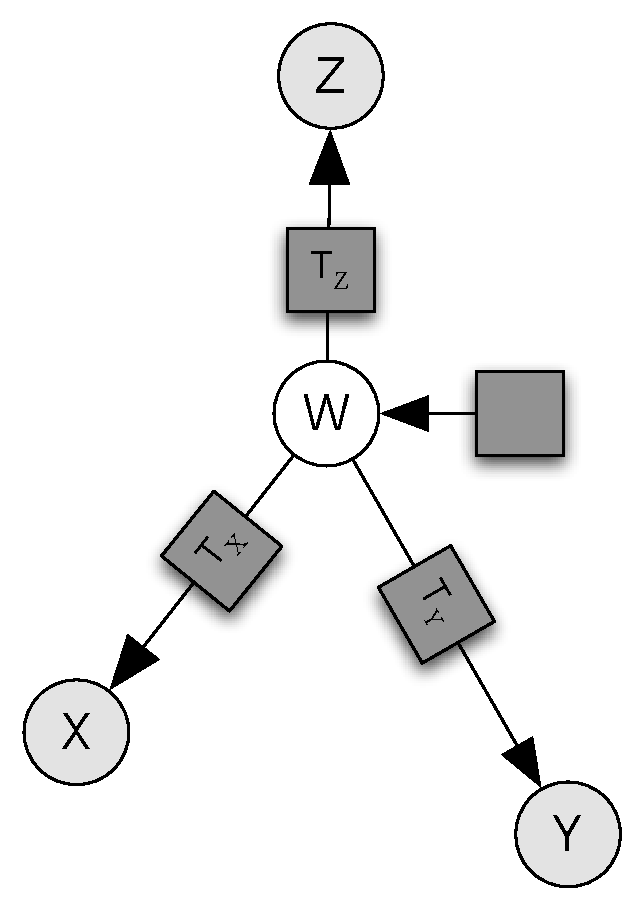
\includegraphics [scale=0.4] {figs/threeway.pdf}
  \caption{\figlabel{threeway}
    A star phylogeny with three (extant) leaf sequences.
    An ancestral sequence $W$ evolves into three descendant sequences $X$, $Y$ and $Z$.
    A singlet transducer (the horizontal gray box) emit ancestral sequence and structure
    and three branch transducers (the gray boxes labeled $\Delta T_X$, $\Delta T_Y$ and $\Delta T_Z$)
    mutate it according to the specified multi-sequence model.
    Gray nodes correspond to observed data and white nodes unobserved data.
    If the branch transducers are time-reversible, then this star phylogeny with three leaves is
    the neighborhood of any interior node in a (binary) phylogenetic tree, 
    from which it follows that evaluating the likelihood function
    on this star phylogeny is sufficient for a sampling algorithm on an arbitrary phylogeny.
  }
\end{figure}

\subsection{Notation}
The 3 (ungapped) sequences to be aligned are $x^{(1)}$, $x^{(2)}$ and $x^{(3)}$
(we refer to them by an index rather than as $X$, $Y$ and $Z$ for notational convenience).
The $\mathrm{i}^{\mathrm{th}}$ symbol of sequence $x^{(1)}$ is written $x^{(1)}_i$ 
and the length of the same sequence is $L_1 = |x^{(1)}|$.


\subsection{Fold Envelopes} \seclabel{foldenv}
We use the fold envelope concept \cite{HolmesRubin2002a,Holmes2004} to constrain the set of structures our algorithms consider.
A fold envelope $\foldenv$ for a sequence $x$ is a set of coordinate pairs satisfying
\beqn \label{eqn:cabbage}
\foldenv \subset \left\{ (i,j):0 \le i \le j \le L \right\} \, .
\eeqn
We consider a subsequence $x_{i+1} \dots x_{j}$ only if the corresponding coordinate pair $(i,j) \in \foldenv$.
The unconstrained fold envelope has set equality in \eqref{eqn:cabbage}.

We use two orderings for sequences in the fold envelopes.  An inside-outside ordering is used for the iteration 
in the Inside algorithm: Subsequences are ordered such that each successive subsequence 
contains all previous subsequences in the fold envelope.  More precisely, subsequences in $\mathscr{F}$ are sorted  
in the same order as coordinate pairs $(i,j)$ are generated by the iteration $\{\,\mathrm{for}\, i = L \,\mathrm{to}\, 0 \,\,\{ \mathrm{for}\, j = i \,\mathrm{to}\, L \}\,\}$.

The Outside algorithm uses an outside-inside ordering, where subsequences starting at a fixed $i$ are reverse-sorted 
with respect to the inside-outside ordering described above.  Subsequences in $\mathscr{F}$ are then sorted 
in the same order as coordinate pairs $(i,j)$ are generated by the 
iteration $\{\,\mathrm{for}\, i = 0 \,\mathrm{to}\, L \,\,\{ \mathrm{for}\, j = L\, \mathrm{to}\, i \}\,\}$.

We frequently refer to subsequences by their index in the fold envelope.
The $\mth$ subsequence in $\foldenv$ is labeled $m$ and corresponds to the coordinate pair $(i_{m}, j_{m})$.  The 
index of a pair $(i,j) \in \foldenv$ is $n[i,j]$.

Inward and outward emission connections, specifying which subsequences are reachable from 
a given subsequence and state, are defined as
\begin{align}
c_{in}\left(\bvec{b}; m\right) &= n\left[ i_{m} + \Delta_{\bvec{b}}^{L}, j_{m} - \Delta_{\bvec{b}}^{R} \right] \\
c_{out}\left(\bvec{b}; m\right) &= n\left[ i_{m} - \Delta_{\bvec{b}}^{L}, j_{m} + \Delta_{\bvec{b}}^{R} \right]
\end{align}
The emission connection is undefined if the corresponding subsequence is not in the fold envelope.\footnote{We defined emission connections slightly differently than do \cite{HolmesRubin2002a}.}  Inward, outward-left and outward-right bifurcation connections are defined as
\begin{align}
b_{in}(n) &= \left\{ \left( n_L,n_R \right): i_{n_L} = i_{n},\, j_{n_L} = i_{n_R},\, j_{n_R} = j_{n} \right\} \\
b_{out,L}(n) &= \left\{ \left( n_O,n_L \right): i_{n_L} = i_{n_O},\, j_{n_L} = i_{n},\, j_{n} = j_{n_O} \right\} \\
b_{out,R}(n) &= \left\{ \left( n_O,n_R \right): i_{n} = i_{n_O},\, j_{n} = i_{n_R},\, j_{n_R} = j_{n_O} \right\}
\end{align}

We generally write out explicit subsequence coordinate pairs $(i,j)$ when their usage will make mathematical formulae clearer and 
fold-envelope labels $n$ when writing pseudocode.  An implementation will rely on such an iterator over subsequences in the fold envelope.

\subsection{Inside}
The inside probability $\inside{\bvec{a}}{i_1}{j_1}{i_2}{j_2}{i_3}{j_3}$ is the summed probability of subsequences 
$x^{(1)}_{i_1+1} \dots x^{(1)}_{j_1}$, $x^{(2)}_{i_2+1} \dots x^{(2)}_{j_2}$, $x^{(3)}_{i_3+1} \dots x^{(3)}_{j_3}$
under all paths through the model which are rooted in state $\bvec{a}$.  
\algref{inside} gives pseudocode for the fold-envelope version of the Inside algorithm.  The subroutines 
$\mathrm{calcTransEmitProb}()$, $\mathrm{calcLBifurcProb}()$ and $\mathrm{calcRBifurcProb}()$
used in the Inside algorithm are defined below.

\begin{algorithm}[!ht]

  \SetKwData{bifurcProb}{bifurcProb}
  \SetKwFunction{calcTransEmitProb}{calcTransEmitProb}
  \SetKwFunction{calcLBifurcProb}{calcLBifurcProb}
  \SetKwFunction{calcRBifurcProb}{calcRBifurcProb}
  \SetLine
  \KwIn{sequences $x^{(1)},x^{(2)},x^{(3)}$}

  initialization\;
  \ForEach(\tcc*[f]{inside-outside sorted}){$n^{(1)} \in \foldenv^{(1)}$} {
    \ForEach(\tcc*[f]{inside-outside sorted}){$n^{(2)} \in \foldenv^{(2)}$} {
      \ForEach(\tcc*[f]{inside-outside sorted}){$n^{(3)} \in \foldenv^{(3)}$} {
        \BlankLine
        \ForEach{state $\bvec{a}$}{
          \BlankLine
          \bifurcProb $\leftarrow 0$\;
          \ForEach{$\left( n^{(1)}_L,n^{(1)}_R \right) \in b_{in}\left( n^{(1)} \right)$} {
            \ForEach{$\left( n^{(2)}_L,n^{(2)}_R \right) \in b_{in}\left( n^{(2)} \right)$} {
              \ForEach{$\left( n^{(3)}_L,n^{(3)}_R \right) \in b_{in}\left( n^{(3)} \right)$} {
                \bifurcProb += \calcLBifurcProb($\bvec{a}; \cdot$)\;
                \bifurcProb += \calcRBifurcProb($\bvec{a}; \cdot$)\;
              }
            }
          }
          \BlankLine
          $\alpha_{\bvec{a}} \left( n^{(1)}, n^{(2)}, n^{(3)} \right)$ $\leftarrow$ \calcTransEmitProb$\left( \bvec{a}; n^{(1)}, n^{(2)}, n^{(3)} \right)$\;
          $\alpha_{\bvec{a}} \left( n^{(1)}, n^{(2)}, n^{(3)} \right)$ += \bifurcProb\;
          store $\alpha_{\bvec{a}} \left( n^{(1)}, n^{(2)}, n^{(3)} \right)$\;
        }
        \BlankLine
      }
    }
  }
  \KwRet{$\alpha_{\bvec{a}}\left( n[0,L_1],n[0,L_2],n[0,L_3] \right)$}\;
  
  \caption{\alglabel{inside}
    The constrained Inside algorithm for three sequences $x^{(1)},x^{(2)},x^{(3)}$.
    States $\bvec{a}$ in the iteration over states are sorted in Inside fill order
    with $\Semit$ states first, then $\Snull$ states in reverse topological order.
  }
\end{algorithm}

The transition and emission probability $\mathrm{calcTransEmitProb}(\bvec{a}; \cdot)$ can be calculated recursively 
in the unconstrained case as
\begin{align} \label{eqn:insidetransemit}
  & \sum_{y_1\in\{x^{(1)}_{i_1+1},\Tnull\}}\sum_{z_1\in\{x^{(1)}_{j_1},\Tnull\}} \sum_{y_2\in\{x^{(2)}_{i_2+1},\Tnull\}}\sum_{z_2\in\{x^{(2)}_{j_2},\Tnull\}} \sum_{y_3\in\{x^{(3)}_{i_3+1},\Tnull\}}\sum_{z_3\in\{x^{(3)}_{j_3},\Tnull\}} \nonumber \\
  &\qquad \left[ \sum_{\bvec{b}|\,\exists\, \bvec{a}\to\bvec{y}\bvec{b}\bvec{z}} \weight (\bvec{a}\to\bvec{y}\,\bvec{b}\,\bvec{z}) \inside{\bvec{b}}{i_1+|y_1|}{j_1-|z_1|}{i_2+|y_2|}{j_2-|z_2|}{i_3+|y_3|}{j_3-|z_3|} \right] . \nonumber
\end{align}
Null transitions are caught in the sum when the terminals $\bvec{y} = \bvec{z} = \Tnull$.
The constrained case is handled differently: The multiple sums are replaced by a single iteration over states $\bvec{b}$
which connect subsequences $n^{(1)}, n^{(2)}, n^{(3)}$ to others in the fold envelopes.
Pseudocode for the constrained calculation is given in \algref{insidetransemit}.

\begin{algorithm}[!ht]
  \SetKwData{emitProb}{emitProb}
  \SetKwFunction{Weight}{Weight}
  \SetLine
  \KwIn{state $\bvec{a}, n^{(1)}, n^{(2)}, n^{(3)}$, intermediate Inside matrix $\alpha$}

  \emitProb $\leftarrow 0$\;
  \ForEach{$\bvec{b} : \exists \,\bvec{a} \to \bvec{b}$} {
    \emitProb += \Weight$\left( \bvec{a} \to \bvec{b} \right)\, \alpha_{\bvec{b}}\left( n^{(1)}, n^{(2)}, n^{(3)} \right)$\;
  }
  \ForEach{$\bvec{b} : \exists \,\bvec{a} \to \bvec{y}\,\bvec{b}\,\bvec{z}$} {
    \lIf{$c_{in}\left(\bvec{b}; n^{(1)}\right) \notin \foldenv^{(1)}$ or $c_{in}\left(\bvec{b}; n^{(2)}\right) \notin \foldenv^{(2)}$ or $c_{in}\left(\bvec{b}; n^{(3)}\right) \notin \foldenv^{(3)}$}{next\;}
    \emitProb += \Weight$\left( \bvec{a} \to \bvec{y}\,\bvec{b}\,\bvec{z} \right)\, \alpha_{\bvec{b}}\left( c_{in}\left(\bvec{b}; n^{(1)}\right), c_{in}\left(\bvec{b}; n^{(2)}\right), c_{in}\left(\bvec{b}; n^{(3)}\right) \right)$\;
  }
  \KwRet{\emitProb}\;
  \caption{\alglabel{insidetransemit}
    Subroutine $\mathrm{calcTransEmitProb}()$ for the Inside algorithm.
  }
\end{algorithm}

The left-bifurcation probability $\mathrm{calcLBifurcProb}\left( \bvec{a}; n^{(1)}_L,n^{(1)}_R,n^{(2)}_L,n^{(2)}_R,n^{(3)}_L,n^{(3)}_R \right)$ is
\[ \sum_{\bvec{b}|\,\exists\, \bvec{a}\to\bvec{c}\bvec{b}} \weight (\bvec{a}\to\bvec{c}\,\bvec{b}) \, \alpha_{\bvec{c}}\left( n^{(1)}_L,n^{(2)}_L,n^{(3)}_L\right) \, \alpha_{\bvec{b}}\left( n^{(1)}_R,n^{(2)}_R,n^{(3)}_R\right) \]
and the right-bifurcation probability $\mathrm{calcRBifurcProb}\left( \bvec{a}; n^{(1)}_L,n^{(1)}_R,n^{(2)}_L,n^{(2)}_R,n^{(3)}_L,n^{(3)}_R \right)$ is
\[ \sum_{\bvec{b}|\,\exists\, \bvec{a}\to\bvec{b}\bvec{d}} \weight (\bvec{a}\to\bvec{b}\,\bvec{d}) \, \alpha_{\bvec{b}}\left( n^{(1)}_L,n^{(2)}_L,n^{(3)}_L\right) \, \alpha_{\bvec{d}}\left( n^{(1)}_R,n^{(2)}_R,n^{(3)}_R\right) . \]

The boundary condition gives the probability of a subsequence of length 0,
\beqn \label{eqn:insidetoend}
\inside{\bvec{a}}{j_1}{j_1}{j_2}{j_2}{j_3}{j_3} = t(\bvec{a},\Send) + \sum_{\bvec{b}|\,\exists\, \bvec{a}\to\bvec{b}} \weight (\bvec{a}\to\bvec{b}) \, \inside{\bvec{a}}{j_1}{j_1}{j_2}{j_2}{j_3}{j_3} \, ,
\eeqn
for $0 \le j_1 \le L_1, 0 \le j_2 \le L_2, 0 \le j_3 \le L_3$.
We are assuming that there are no cycles of $\Snull$ states as well as no bifurcations which can result in no emissions.
The termination condition is 
\[ P\left(x^{(1)},x^{(2)},x^{(3)}\right) = \alpha_{\mathrm{Start}}(0,L_1,0,L_2,0,L_3) \, , \]
where $\mathrm{Start}$ is the unique start state of the model.

We write the DP algorithms using the $\weight (\cdot)$ notation in order to preserve generality: In our formalism, a transition $a \to x\,b$ has $\emit(b) = x$, but the more common convention is to have $\emit(a) = x$.
The difference will show up only in the value assigned to $\weight (a \to x\,b)$, so our DP algorithms can be used in both cases.


\subsection{CYK}
The CYK algorithm can be obtained from the Inside algorithm by replacing sums over paths through the model (or equivalently, parses)
with the $\max()$ operation (e.g., in \eqref{eqn:insidetoend}, $\sum_{\bvec{b}|\,\exists\, \bvec{a}\to\bvec{b}}$ will be replaced by $ \max_{\bvec{b}|\,\exists\, \bvec{a}\to\bvec{b}}$).
The CYK probabilities for indices $(i_1,j_1,i_2,j_2,i_3,j_3)$ then represent 
the probability of the most likely path through the model for 
subsequences $x^{(1)}_{i_1+1} \dots x^{(1)}_{j_1}$, $x^{(2)}_{i_2+1} \dots x^{(2)}_{j_2}$, $x^{(3)}_{i_3+1} \dots x^{(3)}_{j_3}$.


\subsection{Outside}
The outside probability $\outside{\bvec{b}}{i_1}{j_1}{i_2}{j_2}{i_3}{j_3}$ is the summed probability of the sequences $x^{(1)}$, $x^{(2)}$, $x^{(3)}$ 
under all paths through the model which are rooted in the start state of the model, excluding all paths for the subsequences 
$x^{(1)}_{i_1+1} \dots x^{(1)}_{j_1}$, $x^{(2)}_{i_2+1} \dots x^{(2)}_{j_2}$, $x^{(3)}_{i_3+1} \dots x^{(3)}_{j_3}$ 
which are rooted in the state $\bvec{b}$.
\algref{outside} gives pseudocode for the fold-envelope version of the Outside algorithm.
The subroutines $\mathrm{calcTransEmitProb}()$, $\mathrm{calcLBifurcProb}()$ and $\mathrm{calcRBifurcProb}()$
used in the Outside algorithm are defined below.


\begin{algorithm}[!ht]
  \SetKwFunction{calcTransEmitProb}{calcTransEmitProb}
  \SetKwData{bifurcProb}{bifurcProb}
  \SetKwFunction{calcLBifurcProb}{calcLBifurcProb}
  \SetKwFunction{calcRBifurcProb}{calcRBifurcProb}
  \SetLine
  \KwIn{sequences $x^{(1)},x^{(2)},x^{(3)}$, CYK matrix $\alpha$}

  initialization\;
  \ForEach(\tcc*[f]{outside-inside sorted}){$n^{(1)} \in \foldenv^{(1)}$} {
    \ForEach(\tcc*[f]{outside-inside sorted}){$n^{(2)} \in \foldenv^{(2)}$} {
      \ForEach(\tcc*[f]{outside-inside sorted}){$n^{(3)} \in \foldenv^{(3)}$} {
        \BlankLine
        \ForEach{state $\bvec{b}$}{
          \BlankLine
          \bifurcProb $\leftarrow 0$\;
          \ForEach{$\left( n^{(1)}_O,n^{(1)}_L \right) \in b_{out,L}\left( n^{(1)} \right)$}{
            \ForEach{$\left( n^{(2)}_O,n^{(2)}_L \right) \in b_{out,L}\left( n^{(2)} \right)$}{
              \ForEach{$\left( n^{(3)}_O,n^{(3)}_L \right) \in b_{out,L}\left( n^{(3)} \right)$}{
                \bifurcProb += \calcLBifurcProb($\bvec{b}; \cdot$)\;
              }
            }
          }
          \ForEach{$\left( n^{(1)}_O,n^{(1)}_R \right) \in b_{out,R}\left( n^{(1)} \right)$}{
            \ForEach{$\left( n^{(2)}_O,n^{(2)}_R \right) \in b_{out,R}\left( n^{(2)} \right)$}{
              \ForEach{$\left( n^{(3)}_O,n^{(3)}_R \right) \in b_{out,R}\left( n^{(3)} \right)$}{
                \bifurcProb += \calcRBifurcProb($\bvec{b}; \cdot$)\;
              }
            }
          }
          \BlankLine
          $\beta_{\bvec{b}} \left( n^{(1)}, n^{(2)}, n^{(3)} \right) \leftarrow$ \calcTransEmitProb$\left( \bvec{b}; n^{(1)}, n^{(2)}, n^{(3)} \right)$\;
          $\beta_{\bvec{b}} \left( n^{(1)}, n^{(2)}, n^{(3)} \right)$ += \bifurcProb\;
          store $\beta_{\bvec{b}} \left( n^{(1)}, n^{(2)}, n^{(3)} \right)$\;
        }
        \BlankLine
      }
    }
  }
  \caption{\alglabel{outside}
    The constrained Outside algorithm for three sequences $x^{(1)},x^{(2)},x^{(3)}$.
    States $\bvec{a}$ in the iteration over states are sorted in Outside fill order
    with $\Semit$ states first, then $\Snull$ states in topological order.
  }
\end{algorithm}

The transition and emission probability $\mathrm{calcTransEmitProb}()$ can be calculated recursively in the unconstrained case as
\begin{align}
  & \sum_{y_1\in\{x^{(1)}_{i_1},\Tnull\}}\sum_{z_1\in\{x^{(1)}_{j_1+1},\Tnull\}} \sum_{y_2\in\{x^{(2)}_{i_2},\Tnull\}}\sum_{z_2\in\{x^{(2)}_{j_2+1},\Tnull\}} \sum_{y_3\in\{x^{(3)}_{i_3},\Tnull\}}\sum_{z_3\in\{x^{(3)}_{j_3+1},\Tnull\}} \nonumber \\
  & \qquad \left[ \sum_{\bvec{a}|\,\exists\, \bvec{a}\to\bvec{y}\bvec{b}\bvec{z}} \weight (\bvec{a}\to\bvec{y}\,\bvec{b}\,\bvec{z}) \, \outside{\bvec{a}}{i_1-|y_1|}{j_1+|z_1|}{i_2-|y_2|}{j_2+|z_2|}{i_3-|y_3|}{j_3+|z_3|}  \right] . \nonumber
\end{align}
As with the Inside algorithm, an efficient implementation of the fold-envelope constraints requires a different treatment, given in \algref{outsidetransemit}.

The left-bifurcation probability $\mathrm{calcLBifurcProb}\left( \bvec{b}; n^{(1)}_O,n^{(1)}_L,n^{(2)}_O,n^{(2)}_L,n^{(3)}_O,n^{(3)}_L \right)$ is
\[ \sum_{\bvec{a}|\,\exists\, \bvec{a}\to\bvec{c}\bvec{b}} \weight (\bvec{a}\to\bvec{c}\,\bvec{b}) \, \beta_{\bvec{a}}\left( n^{(1)}_O,n^{(2)}_O,n^{(3)}_O\right) \, \alpha_{\bvec{c}}\left( n^{(1)}_L,n^{(2)}_L,n^{(3)}_L\right) \]
and the right-bifurcation probability $\mathrm{calcRBifurcProb}\left( \bvec{b}; n^{(1)}_O,n^{(1)}_R,n^{(2)}_O,n^{(2)}_R,n^{(3)}_O,n^{(3)}_R \right)$ is
\[ \sum_{\bvec{a}|\,\exists\, \bvec{a}\to\bvec{b}\bvec{d}} \weight (\bvec{a}\to\bvec{b}\,\bvec{d}) \, \beta_{\bvec{a}}\left( n^{(1)}_O,n^{(2)}_O,n^{(3)}_O\right) \, \alpha_{\bvec{d}}\left( n^{(1)}_R,n^{(2)}_R,n^{(3)}_R\right) \]


\begin{algorithm}[!ht]
  \SetKwData{emitProb}{emitProb}
  \SetKwFunction{Weight}{Weight}
  \SetLine
  \KwIn{state $\bvec{b}, n^{(1)}, n^{(2)}, n^{(3)}$, intermediate Outside matrix $\beta$}

  \emitProb $\leftarrow 0$\;
  \ForEach{$\bvec{a} : \exists \,\bvec{a} \to \bvec{b}$} {
    \emitProb += \Weight$\left( \bvec{a} \to \bvec{b} \right)\, \beta_{\bvec{a}}\left( n^{(1)}, n^{(2)}, n^{(3)} \right)$\;
  }
  \ForEach{$\bvec{a} : \exists \,\bvec{a} \to \bvec{y}\,\bvec{b}\,\bvec{z}$} {
    \lIf{$c_{out}\left(\bvec{b}; n^{(1)}\right) \notin \foldenv^{(1)}$ or $c_{out}\left(\bvec{b}; n^{(2)}\right) \notin \foldenv^{(2)}$ or $c_{out}\left(\bvec{b}; n^{(3)}\right) \notin \foldenv^{(3)}$}{next\;}
    \emitProb += \Weight$\left( \bvec{a} \to \bvec{y}\,\bvec{b}\,\bvec{z} \right)\, \beta_{\bvec{a}}\left( c_{out}\left(\bvec{b}; n^{(1)}\right), c_{out}\left(\bvec{b}; n^{(2)}\right), c_{out}\left(\bvec{b}; n^{(3)}\right) \right)$\;
  }
  \KwRet{\emitProb}\;
  \caption{\alglabel{outsidetransemit}
    Subroutine $\mathrm{calcTransEmitProb}()$ for the Outside algorithm.
  }
\end{algorithm}

The boundary condition is just
\beqn
\outside{\mathrm{Start}}{0}{L_1}{0}{L_2}{0}{L_3} = 1 \, .
\eeqn



\subsection{Loopy DP}

The standard Inside and Outside algorithms fail on grammars with 1) cycles of $\Snull$ states, 
or 2) bifurcations with empty children
because they are incapable of performing a probabilistic summation over $\Snull$ cycles
(empty children of bifurcations can give rise to effective cycles of $\Snull$ states).
Phrased qualitatively, the standard Inside and Outside fail because the iterations over
states $\bvec{a}$ in \algref{inside} and \algref{outside}
can correspond to, at most, single $\Snull$ cycles rather than the infinitely many which are possible.

While we believe that an efficient analytic summation is impossible,
we can use an iterative approach to approximate an exact result to high precision.
A brute-force approach is to just repeatedly iterate over all states $\bvec{a}$ until
convergence is reached, but this is computationally-costly.
A much more efficient algorithm exists.
The key insight is that only $\Snull$ states which are strongly connected
(reachable from each other in the state graph by either other $\Snull$ states
or bifurcations with empty children) can contribute to any possible $\Snull$ cycle.
It follows that instead of repeatedly iterating over all states $\bvec{a}$,
it suffices to decompose the state (sub) graph of $\Snull$ states and bifurcation
states with possibly-empty children into its strongly-connected components
and repeatedly iterate over these connected components rather than the entire graph.
Decomposition of a graph into its strongly-connected components can
be done in linear time \cite{Tarjan1972},
so the overall complexity of inference is still determined by the DP iterations themselves.
If we iterate over each connected component 5 times, then upper bounds on 
the complexity of inference are
$O(5 \cdot A \cdot L^{2n})$ and $O(5 \cdot A \cdot L^{3n})$ in space and time for a model 
with $A$ states of $n$ extant sequences.
For the star phylogeny of \figref{threeway}, 


\newpage
\section{The TKF Structure Tree model as a transducer} \seclabel{tkfst}

We can cast the TKF91 Structure Tree model as a transducer.
{\bf Why is this important/useful? e.g. ``This means we can automatically deduce rules like those shown in Tables~\tabnum{abc} through~\tabref{agapbc}...''}

\subsection{The single-sequence TKFST model as a singlet transducer}

The states of the singlet transducer are shown in \tabref{tkfstsinglet}.
Allowed transitions between these states are shown in the paper.

\begin{table}[!ht]
  \centering
  \begin{tabular}{lrrrr}
    state & $\type$ & $\absorb$ & $\emit$ & $e(\,\bullet\,|\mathrm{TKFST})$ \\ \hline
    $L$ & $\Sstart$ \\
    $I_L$ & $\Sinsert$ & & $(x,\Tnull)$ & $p(x)$ \\
    \\
    $S$ & $\Sstart$ \\
    $I_S$ & $\Sinsert$ & & $(x,y)$ & $p(x,y)$ \\
    \\
    $B$ & $\Sinsert$ & & $(L\,S)$ & 1 \\
  \end{tabular}
  \caption{
    \tablabel{tkfstsinglet}
    States of the singlet transducer of the TKF Structure Tree model \cite{Holmes2004}.
    Singlet transducers can only have states of type $\Sstart$ or $\Sinsert$.
    {\bf This is the indiegram-style transducer equivalent of the SCFG in \tabref{a} ...}
  }
\end{table}


\subsection{The two-sequence TKFST model as a branch transducer}

The states of the branch transducer are shown in \tabref{tkfstbranch}.
Allowed transitions between these states are shown in the paper.

\begin{table}[!ht]
  \centering
  \begin{tabular}{lrrrr}
    state & $\type$ & $\absorb$ & $\emit$ & $e(\,\bullet\,|\mathrm{TKFST})$ \\ \hline
    $L$ & $\Sstart$ \\
    $I_L$ & $\Sinsert$ & & $(u,\Tnull)$ & $p(u)$ \\
    $M_L$ & $\Smatch$ & $(x,\Tnull)$ & $(u,\Tnull)$ & $p(u|x)$ \\
    $D_L$ & $\Smatch$ & $(x,\Tnull)$ & $(\Tgap,\Tnull)$ & 1 \\
    $W_L$ & $\Swait$ \\
    \\
    $S$ & $\Sstart$ \\
    $I_S$ & $\Sinsert$ & & $(u,v)$ & $p(u,v)$ \\
    $M_S$ & $\Smatch$ & $(x,y)$ & $(u,v)$ & $p(u,v|x,y)$ \\
    $D_S$ & $\Smatch$ & $(x,y)$ & $(\Tgap,\Tgap)$ & 1 \\
    $W_S$ & $\Swait$ \\
    \\
    $B_i$ & $\Sinsert$ & & $(L_i\,S_i)$ & 1 \\
    $B$ & $\Smatch$ & $(L\,S)$ & $(L\,S)$ & 1 \\
    $B_p$ & $\Smatch$ & $(L\,S)$ & $(L\,\Send)$ & 1 \\
    $B_e$ & $\Smatch$ & $(L\,\Send)$ & $(L\,\Send)$ & 1 \\
  \end{tabular}
  \caption{\tablabel{tkfstbranch}
    States of the branch transducer of the TKF Structure Tree model \cite{Holmes2004}.
    States which have the same names as states of the singlet transducer in \tabref{tkfstsinglet}
    are the branch equivalent of the corresponding singlet states
    (e.g. a $\Smatch$ state might be the branch equivalent of an $\Sinsert$ state).
    States $L_i$ and $S_i$ are the $\Sstart$ states of a sub-model (not shown) identical
    in structure to the singlet transducer.  They are used to insert a new stem-loop structure.
    {\bf This is the indiegram-style transducer equivalent of the SCFG in \tabref{ab} ...}
  }
\end{table}




\subsection{The multi-sequence TKFST model as a composite transducer}

We can use the state graph construction algorithm described 
in the paper and detailed in \secref{stategraph} to create a model of the simultaneous evolution
of several sequences.

\begin{figure}[!htb]
  \centering
  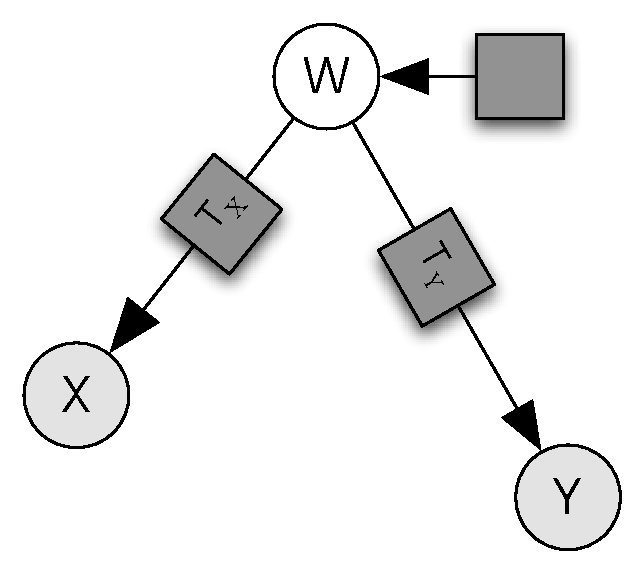
\includegraphics [scale=0.4] {figs/parent.pdf}
  \caption{\figlabel{parent}
    A simple example of transducer composition to build a multi-sequence model of two extant sequences.
    An ancestral sequence $W$ evolves into two descendant sequences $X$ and $Y$.
    A singlet transducer (the horizontal gray box) emit ancestral sequence and structure
    and two branch transducers (the gray boxes labeled $\Delta T_X$ and $\Delta T_Y$)
    mutate it according to the specified multi-sequence model.
    Gray nodes correspond to observed data and white nodes unobserved data.
  }
\end{figure}

Consider the simple model shown in \figref{parent}.
The state of the multi-sequence model describing this model is a 3-vector $\bvec{a} = \left( a_1,\,a_2,\,a_3 \right)$,
where $a_1$ is the state of the singlet transducer generating the ancestral sequence $W$
and $a_2$ and $a_3$ are the states of the branch transducers evolving $W$ into
extant sequences $X$ and $Y$.

We can show some of the allowed transitions of this multi-sequence model.
The state of the branch transducer associated with the active node $n$ is shown in bold.

\paragraph{Stem creation.}

A stem is created at the root node $W$ (corresponding to a bifurcation in the singlet transducer $a_1$)
and survives in the sequence $X$ at node 2 but is deleted in the sequence $Y$ at node 3.

\begin{align}
  \nakedthreevec{1:}{2:}{3:} \quad
  \threevec{L}{L}{\mathbf{L}} &
  \to \threevec{\mathbf{L}}{W_L}{W_L}
  \to \threevec{B}{B}{B_p}
  \to \threevec{L}{L}{\mathbf{L}} \, \threevec{S}{\mathbf{S}}{\Send}
  \to \threevec{L}{L}{\mathbf{L}} \, \threevec{\mathbf{S}}{W_S}{\Send} \\
  & \to \threevec{\mathbf{L}}{W_L}{W_L} \, \threevec{\mathbf{S}}{W_S}{\Send}
\end{align}


\paragraph{Stem insertion.}

A stem sequence is inserted in sequence $X$ at node 2.

\begin{align}
  \nakedthreevec{1:}{2:}{3:} \quad
  \threevec{L}{L}{\mathbf{L}} \to \threevec{L}{\mathbf{L}}{W_L}
  \to \threevec{L}{B_i}{B}
  \to \threevec{L}{L}{\mathbf{L}} \, \threevec{\Send}{S}{\mathbf{S}}
  \to \threevec{\mathbf{L}}{W_L}{W_L} \, \threevec{\Send}{\mathbf{S}}{W_S}
\end{align}

\paragraph{Stem termination.}

All stem sequences are ended by (possibly empty) loop sequences.

\begin{align}
  \nakedthreevec{1:}{2:}{3:} \quad
  \threevec{\mathbf{S}}{W_S}{W_S}
  \to \threevec{B_e}{B_e}{B_e}
  \to \threevec{\Send}{\Send}{\Send} \, \threevec{L}{L}{\mathbf{L}}
  \to \threevec{\Send}{\Send}{\Send} \, \threevec{\Send}{\Send}{\Send}
\end{align}


The functions $\alpha(t)$, $\beta(t)$ and $\gamma(t)$ are parametrized by the insertion and deletion rates of the Structure Tree model.
They are defined for loop sequences as
\begin{align}
  \kappa_1 &= \lambda_1 / \mu_1 \\
  \alpha_1 &= \exp \left( -\mu_1 t \right) \\
  \beta_1 &= \frac{\lambda_1 \left( 1 - \exp \left((\lambda_1 - \mu_1) t \right) \right)}{\mu_1 - \lambda_1 \exp \left( (\lambda_1 - \mu_1) t \right) } \\
  \gamma_1 &= 1 - \frac{\mu_1 \left( 1 - \exp \left((\lambda_1 - \mu_1) t \right) \right)}{\left( 1 - \exp (- \mu_1 t) \right) \left(\mu_1 - \lambda_1 \exp \left( (\lambda_1 - \mu_1) t \right) \right) }
\end{align}
and similarly for stem sequences \cite{Holmes2004}.


\newpage
% TKF Structure Tree: Pair SCFGs & parameterizations.
% Summarized from rnaevol-paper/rnaevol.tex  by IH, 12/9/2008

\newcommand\gap{\ast}

\newcommand\ruletable[3]{
\begin{tabular}{rcc|rrr}
\multicolumn{6}{l}{\em #1} \\
\multicolumn{6}{l}{\em #2}\\
#3
\end{tabular}
}
\newcommand\tkfstruletable[3]{\ruletable{TKF Structure Tree #1}{#2}{#3}}

\newcommand\lhsrhs[5]{ #1 & $\to$ & #2 & #3 & #4 & #5 \\ }
\newcommand\rhs[4]{       &   $|$ & #1 & #2 & #3 & #4 \\ }
\newcommand\blank{ & & & & & \\ }


\newcommand\singletgrammar[3]{
% #1 = tree node identifier
% #2 = 5' terminal (left)
% #3 = 3' terminal (right)
\tkfstruletable{singlet rules ($#1$)}
{Sequence $#1$ terminals: $\{ #2, #3 \}$.}
{
\lhsrhs{ lhs }{ rhs }{ $P(#1)$ }{  }{  }
\hline

\blank
\lhsrhs{ $L_{#1}$ }{ ${#2}\ L_{#1}$ }{ $\kappa_l \pi_l(#2)$ }{  }{  }
\rhs{ $S_{#1}\ L_{#1}$ }{ $\kappa_l \pi_l(S)$ }{  }{  }

\rhs{ $\epsilon$ }{ $1-\kappa_l$ }{  }{  }

\blank
\lhsrhs{ $S_{#1}$ }{ ${#2}\ S_{#1}\ {#3}$ }{ $\kappa_s \pi_s(#2#3)$ }{  }{  }
\rhs{ $L_{#1}$ }{ $1-\kappa_s$ }{  }{  }
}
}  % end \singletgrammar



\newcommand\pairgrammar[7]{
% #1 = ancestor
% #2 = descendant
% #3 = ancestral 5' terminal (left)
% #4 = ancestral 3' terminal (right)
% #5 = descendant 5' terminal (left)
% #6 = descendant 3' terminal (right)
% #7 = time suffix (empty string "", apostrophe "'", branch superscript "^{...}")
\tkfstruletable{pair rules ($#1 \stackrel{t#7}{\to} #2$)}
{Sequence $#1$ terminals: $\{ #3, #4 \}$. \quad  Sequence $#2$ terminals: $\{ #5, #6 \}$.}
{
\lhsrhs{ lhs }{ rhs }{ $P(#1)$ }{ $P(#2|#1)$ }{  }
\hline

\blank
\lhsrhs{ $L_{#1#2}$ }{ ${#3}\ {#5}\ L_{#1#2}$ }{ $\kappa_l \pi_l(#3)$ }{ $(1-\beta#7_l) \alpha#7_l M#7_l(#3,#5)$ }{  }
\rhs{ ${#5}\ L_{#1#2}$ }{ $1$ }{ $\beta#7_l \pi_l(#5)$ }{  }
\rhs{ ${#3}\ L_{#1\gap #2}$ }{ $\kappa_l \pi_l(#3)$ }{ $(1-\beta#7_l) (1-\alpha#7_l)$ }{  }

\blank
\rhs{ $S_{#1#2}\ L_{#1#2}$ }{ $\kappa_l \pi_l(S)$ }{ $(1-\beta#7_l) \alpha#7_l$ }{  }
\rhs{ $S_{#2}\ L_{#1#2}$ }{ $1$ }{ $\beta#7_l \pi_l(S)$ }{  }
\rhs{ $S_{#1}\ L_{#1\gap #2}$ }{ $\kappa_l \pi_l(S)$ }{ $(1-\beta#7_l) (1-\alpha#7_l)$ }{  }

\rhs{ $\epsilon$ }{ $1-\kappa_l$ }{ $1-\beta#7_l$ }{  }

\blank
\lhsrhs{ $S_{#1#2}$ }{ ${#3}\ {#5}\ S_{#1#2}\ {#6}\ {#4}$ }{ $\kappa_s \pi_s(#3#4)$ }{ $(1-\beta#7_s)  \alpha#7_s M#7_s(#3#4,#5#6)$ }{  }
\rhs{ ${#5}\ S_{#1#2}\ {#6}$ }{ $1$ }{ $\beta#7_s \pi_s(#5#6)$ }{  }
\rhs{ ${#3}\ S_{#1\gap #2}\ {#4}$ }{ $\kappa_s \pi_s(#3#4)$ }{ $(1-\beta#7_s) (1-\alpha#7_s)$ }{  }
\rhs{ $L_{#1#2}$ }{ $1-\kappa_s$ }{ $1-\beta#7_s$ }{  }

\blank
\lhsrhs{ $L_{#1\gap #2}$ }{ ${#3}\ {#5}\ L_{#1#2}$ }{ $\kappa_l \pi_l(#3)$ }{ $(1-\gamma#7_l) \alpha#7_l M#7_l(#3,#5)$ }{  }
\rhs{ ${#5}\ L_{#1#2}$ }{ $1$ }{ $\gamma#7_l \pi_l(#5)$ }{  }
\rhs{ ${#3}\ L_{#1\gap #2}$ }{ $\kappa_l \pi_l(#3)$ }{ $(1-\gamma#7_l) (1-\alpha#7_l)$ }{  }

\blank
\rhs{ $S_{#1#2}\ L_{#1#2}$ }{ $\kappa_l \pi_l(S)$ }{ $(1-\gamma#7_l) \alpha#7_l$ }{  }
\rhs{ $S_{#2}\ L_{#1#2}$ }{ $1$ }{ $\gamma#7_l \pi_l(S)$ }{  }
\rhs{ $S_{#1}\ L_{#1\gap #2}$ }{ $\kappa_l \pi_l(S)$ }{ $(1-\gamma#7_l) (1-\alpha#7_l)$ }{  }

\rhs{ $\epsilon$ }{ $1-\kappa_l$ }{ $1-\gamma#7_l$ }{  }

\blank
\lhsrhs{ $S_{#1\gap #2}$ }{ ${#3}\ {#5}\ S_{#1#2}\ {#6}\ {#4}$ }{ $\kappa_s \pi_s(#3#4)$ }{ $(1-\gamma#7_s) \alpha#7_s M#7_s(#3#4,#5#6)$ }{  }
\rhs{ ${#5}\ S_{#1#2}\ {#6}$ }{ $1$ }{ $\gamma#7_s \pi_s(#5#6)$ }{  }
\rhs{ ${#3}\ S_{#1\gap #2}\ {#4}$ }{ $\kappa_s \pi_s(#3#4)$ }{ $(1-\gamma#7_s) (1-\alpha#7_s)$ }{  }
\rhs{ $L_{#1#2}$ }{ $1-\kappa_s$ }{ $1-\gamma#7_s$ }{  }
}
}  % end \pairgrammar




\newcommand\abc{$a \stackrel{t}{\to} b \stackrel{t'}{\to} c$}
\newcommand\ab{$a \stackrel{t}{\to} b$}
\newcommand\bc{$b \stackrel{t'}{\to} c$}
\newcommand\ac{$a \stackrel{t+t'}{\longrightarrow} c$}

\newcommand\agapbc{a\gap bc}
\newcommand\abgapc{ab\gap c}

\newcommand\abcstates{``$abc$'' states (post emission at $c$)}
\newcommand\abgapcstates{``$\abgapc$'' states (post deletion on \bc\ branch)}
\newcommand\agapbcstates{``$\agapbc$'' states (post deletion on \ab\ branch)}




\subsection*{The TKFST model on a two-branch phylogeny}

While the idea of composing conditionally-normalized models on a tree
is intuitive, the resulting models can quickly become too complex to
deal with by hand, necessitating an algorithm for automated model
construction.  We constructed the model corresponding to TKFST on the
simple the two-branch phylogeny \abc.
The results, shown below, make clear that by-hand model construction
quickly becomes impractical as model complexity or tree size
increases.

We explicitly note cases where certain sets of grammar rules can be derived
``automatically'' from simpler sets, motivating the development of our
generic tree transducer composition algorithm.


\subsubsection*{Time-dependent probabilities}

Here $n \in \{ l, s \}$ denotes the type of structural element (loop or stem).
${\bf R}^{(n)}$ is the rate matrix and $\pi_n$ the equilibrium distribution.
$\lambda_n$ is the insertion rate and $\mu_n$ is the deletion rate.

\begin{eqnarray*}
\alpha_n(t) & = & \exp (-\mu_n t) \\
\beta_n(t)  & = & \frac {\lambda_n (1 - \exp((\lambda_n-\mu_n)t))} {\mu_n - \lambda_n \exp((\lambda_n-\mu_n)t)} \\
\gamma_n(t) & = & 1 - \frac {\mu_n (1 - \exp((\lambda_n-\mu_n)t))} {(1 - \exp(-\mu_n t))(\mu_n - \lambda_n \exp((\lambda_n-\mu_n)t))}\\
\kappa_n(t) & = & \lambda_n / \mu_n \\
M_n(i,j;t)  & = & \exp({\bf R}^{(n)} t)_{ij}
\end{eqnarray*}

Let $\alpha_n \equiv \alpha_n(t)$ and $\alpha'_n = \alpha_n(t')$; similarly $\beta'_n,\gamma'_n,M'_n$.

\subsubsection*{Grammars}

Note that any of the grammars can be ``downsized'' to a smaller number of sequences, simply by dropping terminals,
yielding alternative applications for each grammar.

For example, the Pair SCFG for \ab\ becomes a Single SCFG for $a$ if sequence $b$ is dropped by removing terminals $w,x$.
Stochastic traceback then can be used to sample the descendant $b$.
This corresponds to a forward-time simulator when we apply the Inside
\& stochastic traceback algorithms.

Similarly, \abc\ can be viewed as a pair grammar \ac\ that can be used
to sample an unknown evolutionary intermediate $b$. Again, this
requires only the Inside \& stochastic traceback algorithms.

% singlet grammars
\paragraph{Singlet rules.}

This section contains three singlet grammars, one for each of the sequences $a$, $b$ and $c$.

Note that Tables~\tabnum{b} and~\tabnum{c} may be deduced automatically from Table~\tabnum{a}
if it is known that the underlying process is initially at equilibrium.

\paragraph{Pair rules.}
% pair grammars

This section contains two pairwise rule-sets.

The pair grammar for \ab\ is the union of Tables~\tabnum{a}, \tabnum{b} and~\tabnum{ab}.

The pair grammar for \bc\ is the union of Tables~\tabnum{b}, \tabnum{c} and~\tabnum{bc}.


Note that \tabref{bc} may be deduced automatically from \tabref{ab}
if it is known that the underlying process is stationary.


\paragraph{Triplet rules.}
% triplet grammar

Because of its length, we have split the triplet rule-set over three tables:
\begin{description}
\item[\tabref{abc}:] Rules for transforming $\{ L_{abc}, S_{abc}\}$ , after emissions to $c$;
\item[\tabref{abgapc}:] Rules for transforming $\{ L_{\abgapc}, S_{\abgapc}\}$ , after deletions on \bc;
\item[\tabref{agapbc}:] Rules for transforming $\{ L_{\agapbc}, S_{\agapbc}\}$ , after deletions on \ab.
\end{description}

The triplet grammar for \abc\ is the union of Tables~\tabnum{a} through~\tabnum{agapbc}.


Note that Tables~\tabnum{abc} through~\tabnum{agapbc} may be deduced automatically from Tables~\tabnum{a} through~\tabnum{bc},
{\bf regardless of the properties of the underlying process,}
using the tree transducer composition algorithm.


% TABLES

% a
\begin{table}
\begin{center}
\singletgrammar{a}{u}{v}
\caption{\tablabel{a} Singlet rule-set for $a$.}
\end{center}
\end{table}
% b
\begin{table}
\begin{center}
\singletgrammar{b}{w}{x}
\caption{\tablabel{b} Singlet rule-set for $b$.}
\end{center}
\end{table}
% c
\begin{table}
\begin{center}
\singletgrammar{c}{y}{z}
\caption{\tablabel{c} Singlet rule-set for $c$.}
\end{center}
\end{table}

%  t
% a->b
\begin{table}
\begin{center}
\pairgrammar{a}{b}{u}{v}{w}{x}{}
\caption{\tablabel{ab} Pair rule-set for \ab\ branch. Requires \tabref{a} and \tabref{b}.}
\end{center}
\end{table}


%  t'
% b->c
\begin{table}
\begin{center}
\pairgrammar{b}{c}{w}{x}{y}{z}{'}
\caption{\tablabel{bc} Pair rule-set for \bc\ branch. Requires \tabref{b} and \tabref{c}.}
\end{center}
\end{table}

%  t  t'
% a->b->c
\newcommand\termdefs{Sequence $a$ terminals: $\{ u, v \}$. \quad Sequence $b$ terminals: $\{ w, x \}$. \quad Sequence $c$ terminals: $\{ y, z \}$.}
\newcommand\tripletheader{\lhsrhs{ lhs }{ rhs }{ $P(a)$ }{ $P(b|a)$ }{ $P(c|b)$ } \hline}

\begin{table}
\begin{center}
\tkfstruletable{triplet rules (\abc): \abcstates}{\termdefs}{\tripletheader
\lhsrhs{ $L_{abc}$ }{ $u\ w\ y\ L_{abc}$ }{ $\kappa_l \pi_l(u)$ }{ $(1-\beta_l) \alpha_l M_l(u,w)$ }{ $(1-\beta'_l) \alpha'_l M'_l(w,y)$}
\rhs{ $ y\ L_{abc}$ }{ $1$ }{ $1$ }{ $\beta'_l \pi_l(y)$}
\rhs{ $ w\ y\ L_{abc}$ }{ $1$ }{ $\beta_l \pi_l(w)$ }{ $(1-\beta'_l) \alpha'_l M'_l(w,y)$}
\rhs{ $ w\ L_{\abgapc}$ }{ $1$ }{ $\beta_l \pi_l(w)$ }{ $(1-\beta'_l) (1-\alpha'_l)$}
\rhs{ $u\ w\ L_{\abgapc}$ }{ $\kappa_l \pi_l(u)$ }{ $(1-\beta_l) \alpha_l M_l(u,w)$ }{ $(1-\beta'_l) (1-\alpha'_l)$}
\rhs{ $u\ L_{\agapbc}$ }{ $\kappa_l \pi_l(u)$ }{ $(1-\beta_l) (1-\alpha_l)$ }{ $1-\beta'_l$}

\blank
\rhs{ $S_{abc}\ L_{abc}$ }{ $\kappa_l \pi_l(S)$ }{ $(1-\beta_l) \alpha_l$ }{ $(1-\beta'_l) \alpha'_l$}
\rhs{ $S_c\ L_{abc}$ }{ $1$ }{ $1$ }{ $\beta'_l \pi_l(S)$}
\rhs{ $S_{bc}\  L_{abc}$ }{ $1$ }{ $\beta_l \pi_l(S)$ }{ $(1-\beta'_l) \alpha'_l$}
\rhs{ $S_b\ L_{\abgapc}$ }{ $1$ }{ $\beta_l \pi_l(S)$ }{ $(1-\beta'_l) (1-\alpha'_l)$}
\rhs{ $S_{ab}\  L_{\abgapc}$ }{ $\kappa_l \pi_l(S)$ }{ $(1-\beta_l) \alpha_l$ }{ $(1-\beta'_l) (1-\alpha'_l)$}
\rhs{ $S_a\ L_{\agapbc}$ }{ $\kappa_l \pi_l(S)$ }{ $(1-\beta_l) (1-\alpha_l)$ }{ $1-\beta'_l$}

\rhs{ $\epsilon$ }{ $1-\kappa_l$ }{ $1-\beta_l$ }{ $1-\beta'_l$}

\blank
\lhsrhs{ $S_{abc}$ }{ $u\ w\ y\ S_{abc}\ z\ x\ v$ }{ $\kappa_s \pi_s(uv)$ }{ $(1-\beta_s)  \alpha_s M_s(uv,wx)$ }{ $(1-\beta'_s)  \alpha'_s M'_s(wx,yz)$}
\rhs{ $y\ S_{abc}\ z$ }{ $1$ }{ $1$ }{ $\beta'_s \pi_s(yz)$}
\rhs{ $w\ y\ S_{abc}\ z\ x$ }{ $1$ }{ $\beta_s \pi_s(wx)$ }{ $(1-\beta'_s)  \alpha'_s M'_s(wx,yz)$}
\rhs{ $w\ S_{\abgapc}\ x$ }{ $1$ }{ $\beta_s \pi_s(wx)$ }{ $(1-\beta'_s)  (1 - \alpha'_s) $}
\rhs{ $u\ w\ S_{\abgapc}\ x\ v$ }{ $\kappa_s \pi_s(uv)$ }{ $(1-\beta_s)  \alpha_s M_s(uv,wx)$ }{ $(1-\beta'_s)  (1-\alpha'_s) $}
\rhs{ $u\ S_{\agapbc}\ v$ }{ $\kappa_s \pi_s(uv)$ }{ $(1-\beta_s) (1-\alpha_s) $ }{ $1-\beta'_s $}

\rhs{ $L_{abc}$ }{ $1-\kappa_s$ }{ $1-\beta_s$ }{ $1-\beta'_s$}
}
\caption{\tablabel{abc} Triplet rule-set for \abcstates\ on \abc\ tree. Requires Tables~\tabnum{a} through~\tabnum{agapbc}.}
\end{center}
\end{table}

\begin{table}
\begin{center}
\tkfstruletable{triplet rules (\abc): \abgapcstates}{\termdefs}{\tripletheader
\lhsrhs{ $L_{\abgapc}$ }{ $u\ w\ y\ L_{abc}$ }{ $\kappa_l \pi_l(u)$ }{ $(1-\beta_l) \alpha_l M_l(u,w)$ }{ $(1-\gamma'_l) \alpha'_l M'_l(w,y)$}
\rhs{ $ y\ L_{abc}$ }{ $1$ }{ $1$ }{ $\gamma'_l \pi_l(y)$}
\rhs{ $ w\ y\ L_{abc}$ }{ $1$ }{ $\beta_l \pi_l(w)$ }{ $(1-\gamma'_l) \alpha'_l M'_l(w,y)$}
\rhs{ $ w\ L_{\abgapc}$ }{ $1$ }{ $\beta_l \pi_l(w)$ }{ $(1-\gamma'_l) (1-\alpha'_l)$}
\rhs{ $u\ w\ L_{\abgapc}$ }{ $\kappa_l \pi_l(u)$ }{ $(1-\beta_l) \alpha_l M_l(u,w)$ }{ $(1-\gamma'_l) (1-\alpha'_l)$}
\rhs{ $u\ L_{\agapbc}$ }{ $\kappa_l \pi_l(u)$ }{ $(1-\beta_l) (1-\alpha_l)$ }{ $1-\gamma'_l$}

\blank
\rhs{ $S_{abc}\ L_{abc}$ }{ $\kappa_l \pi_l(S)$ }{ $(1-\beta_l) \alpha_l$ }{ $(1-\gamma'_l) \alpha'_l$}
\rhs{ $S_c\ L_{abc}$ }{ $1$ }{ $1$ }{ $\gamma'_l \pi_l(S)$}
\rhs{ $S_{bc}\  L_{abc}$ }{ $1$ }{ $\beta_l \pi_l(S)$ }{ $(1-\gamma'_l) \alpha'_l$}
\rhs{ $S_b\ L_{\abgapc}$ }{ $1$ }{ $\beta_l \pi_l(S)$ }{ $(1-\gamma'_l) (1-\alpha'_l)$}
\rhs{ $S_{ab}\  L_{\abgapc}$ }{ $\kappa_l \pi_l(S)$ }{ $(1-\beta_l) \alpha_l$ }{ $(1-\gamma'_l) (1-\alpha'_l)$}
\rhs{ $S_a\ L_{\agapbc}$ }{ $\kappa_l \pi_l(S)$ }{ $(1-\beta_l) (1-\alpha_l)$ }{ $1-\gamma'_l$}

\rhs{ $\epsilon$ }{ $1-\kappa_l$ }{ $1-\beta_l$ }{ $1-\gamma'_l$}

\blank
\lhsrhs{ $S_{\abgapc}$ }{ $u\ w\ y\ S_{abc}\ z\ x\ v$ }{ $\kappa_s \pi_s(uv)$ }{ $(1-\beta_s)  \alpha_s M_s(uv,wx)$ }{ $(1-\gamma'_s)  \alpha'_s M'_s(wx,yz)$}
\rhs{ $y\ S_{abc}\ z$ }{ $1$ }{ $1$ }{ $\gamma'_s \pi_s(yz)$}
\rhs{ $w\ y\ S_{abc}\ z\ x$ }{ $1$ }{ $\beta_s \pi_s(wx)$ }{ $(1-\gamma'_s)  \alpha'_s M'_s(wx,yz)$}
\rhs{ $w\ S_{\abgapc}\ x$ }{ $1$ }{ $\beta_s \pi_s(wx)$ }{ $(1-\gamma'_s)  (1 - \alpha'_s) $}
\rhs{ $u\ w\ S_{\abgapc}\ x\ v$ }{ $\kappa_s \pi_s(uv)$ }{ $(1-\beta_s)  \alpha_s M_s(uv,wx)$ }{ $(1-\gamma'_s)  (1-\alpha'_s) $}
\rhs{ $u\ S_{\agapbc}\ v$ }{ $\kappa_s \pi_s(uv)$ }{ $(1-\beta_s) (1-\alpha_s) $ }{ $1-\gamma'_s $}

\rhs{ $L_{abc}$ }{ $1-\kappa_s$ }{ $1-\beta_s$ }{ $1-\gamma'_s$}
}
\caption{\tablabel{abgapc} Triplet rule-set for \abgapcstates\ on \abc\ tree.  Requires Tables~\tabnum{a} through~\tabnum{agapbc}.}
\end{center}
\end{table}

\begin{table}
\begin{center}
\tkfstruletable{triplet rules (\abc): \agapbcstates}{\termdefs}{\tripletheader
\lhsrhs{ $L_{\agapbc}$ }{ $u\ w\ y\ L_{abc}$ }{ $\kappa_l \pi_l(u)$ }{ $(1-\gamma_l) \alpha_l M_l(u,w)$ }{ $ \alpha'_l M'_l(w,y)$}
\rhs{ $ w\ y\ L_{abc}$ }{ $1$ }{ $\gamma_l \pi_l(w)$ }{ $ \alpha'_l M'_l(w,y)$}
\rhs{ $ w\ L_{\abgapc}$ }{ $1$ }{ $\gamma_l \pi_l(w)$ }{ $ 1-\alpha'_l$}
\rhs{ $u\ w\ L_{\abgapc}$ }{ $\kappa_l \pi_l(u)$ }{ $(1-\gamma_l) \alpha_l M_l(u,w)$ }{ $ 1-\alpha'_l$}
\rhs{ $u\ L_{\agapbc}$ }{ $\kappa_l \pi_l(u)$ }{ $(1-\gamma_l) (1-\alpha_l)$ }{ $1$}

\blank
\rhs{ $S_{abc}\ L_{abc}$ }{ $\kappa_l \pi_l(S)$ }{ $(1-\gamma_l) \alpha_l$ }{ $ \alpha'_l$}
\rhs{ $S_{bc}\  L_{abc}$ }{ $1$ }{ $\gamma_l \pi_l(S)$ }{ $ \alpha'_l$}
\rhs{ $S_b\ L_{\abgapc}$ }{ $1$ }{ $\gamma_l \pi_l(S)$ }{ $ 1-\alpha'_l$}
\rhs{ $S_{ab}\  L_{\abgapc}$ }{ $\kappa_l \pi_l(S)$ }{ $(1-\gamma_l) \alpha_l$ }{ $ 1-\alpha'_l$}
\rhs{ $S_a\ L_{\agapbc}$ }{ $\kappa_l \pi_l(S)$ }{ $(1-\gamma_l) (1-\alpha_l)$ }{ $1$}

\rhs{ $\epsilon$ }{ $1-\kappa_l$ }{ $1-\gamma_l$ }{ $1$}

\blank
\lhsrhs{ $S_{\agapbc}$ }{ $u\ w\ y\ S_{abc}\ z\ x\ v$ }{ $\kappa_s \pi_s(uv)$ }{ $(1-\gamma_s)  \alpha_s M_s(uv,wx)$ }{ $  \alpha'_s M'_s(wx,yz)$}
\rhs{ $w\ y\ S_{abc}\ z\ x$ }{ $1$ }{ $\gamma_s \pi_s(wx)$ }{ $  \alpha'_s M'_s(wx,yz)$}
\rhs{ $w\ S_{\abgapc}\ x$ }{ $1$ }{ $\gamma_s \pi_s(wx)$ }{ $  1 - \alpha'_s $}
\rhs{ $u\ w\ S_{\abgapc}\ x\ v$ }{ $\kappa_s \pi_s(uv)$ }{ $(1-\gamma_s)  \alpha_s M_s(uv,wx)$ }{ $  1-\alpha'_s $}
\rhs{ $u\ S_{\agapbc}\ v$ }{ $\kappa_s \pi_s(uv)$ }{ $(1-\gamma_s) (1-\alpha_s) $ }{ $1$ }

\rhs{ $L_{abc}$ }{ $1-\kappa_s$ }{ $1-\gamma_s$ }{ $1$}
}
\caption{\tablabel{agapbc} Triplet rule-set for \agapbcstates\ on \abc\ tree.  Requires Tables~\tabnum{a} through~\tabnum{agapbc}.}
\end{center}
\end{table}



\newpage
\section{Software}

We have written software tools in Perl and C++ implementing much of the theory described here.
All tools are available from \darturl\ as part of the \dart\ software package for sequence analysis.

\subsection{Automated grammar construction}
We implemented our model construction algorithm on the star phylogeny (\figref{threeway}) 
in a set of Perl scripts.
Given a singlet transducer modeling ancestral sequences and structures and
a branch transducer modeling structural evolution,
the scripts generate C++ code to create the corresponding jointly-normalized SCFG.
All possible models of structural evolution which can be represented by a Pair SCFG
are permitted as input to the scripts,
allowing for flexible and automated model design.

Given files describing the singlet and branch transducers,
including weights of all transitions which may be functions of evolutionary distance,
the package ComposedTreeTransducer::FourWayComposedTT can automatically generate
the state graph and transition matrix of a multi-sequence model of three extant sequences
(\figref{threeway}).
It removes the useless windback $\Snull$ states described in the paper and
introduces effective direct transitions caused by bifurcations with possibly-empty children.
The package ComposedTreeTransducer::TripletSCFG transforms a multi-sequence
model created by ComposedTreeTransducer::FourWayComposedTT into the 
corresponding jointly-normalized three-sequence SCFG (\secref{multigrammars})
and generates C++ code to build the model.

Example singlet and branch transducers files are provided for a simple 
Pair HMM model, a simple Pair SCFG model and the full TKF Structure Tree model.

\subsection{Reconstruction of ancestral structures}
The program \indiegram\ can perform maximum-likelihood inference on the
three-sequence SCFGs automatically generated by the ComposedTreeTransducer::TripletSCFG package.
Complete or no structural information for the three extant sequences can be supplied
as input.


\newpage
\section{Reconstruction of covariant substitution histories}

Our \xrate\ program is a multiple-alignment analysis tool
that estimates rate parameters for a broad class of models, including covariant RNA substitution models \cite{KlostermanEtAl2006}.
It can also be used to predict consensus secondary structures for alignments.
We implemented ancestral sequence reconstruction in \xrate, including posterior probabilities that the reconstructions are correct.

Given a multiple sequence alignment and a phylogenetic tree,
\xrate\ estimates maximum-likelihood values of rate and probability parameters by Expectation Maximization.
During parameter estimation, any unspecified ancestral sequences are summed out using Felsenstein's peeling algorithm.
The new feature is that the program can now find the ancestral sequence that has the highest posterior probability,
contingent on the maximum-likelihood estimates of the model parameters.
During the parameter estimation and ancestral reconstruction steps, the secondary structure may be specified, or it may be summed out as a latent variable.

For the ancestral reconstruction experiments described here,
we assumed that alignment, phylogeny and secondary structure were known,
but that ancestral sequences were unknown.

A simple computational experiment demonstrates the need for covariant substitution models.
We first used \xrate\ to estimate maximum-likelihood parameters for a covariant model of RNA base-pair substitution.
These rates were estimated from ribosomal RNA alignments
derived by \cite{DowellEddy2006} from the European rRNA database \cite{WuytsEtAl2004}.
We also fit a ``naive'' general reversible point-substitution model to these alignments, again using \xrate.
All subsequent results are implicitly conditioned on these maximum-likelihood rate estimates.
Next, we used the companion program SIMGRAM to generate 5000 random alignments (including ancestral sequence),
simulating on a 75-taxon phylogeny from an RNA gene family in the \RFAM\ database \cite{GriffithsJonesEtAl2003}.
(Specifically, we chose the type-I Hammerhead ribozyme, one of the 5\% most populous \RFAM\ families.
 We repeated this experiment with other \RFAM\ phylogenies, but the general trends reported here were not dependent on the choice of tree.)
We stripped the ancestral sequence out of the simulated alignments (leaving the true structure annotation intact),
then re-estimated the ancestral sequence with \xrate, using both the (correct) covariant substitution model and the (naive) non-covariant point-substitution model.
The imputed ancestral sequences were compared to the true sequences (known from the simulation),
and the model-derived posterior probabilities were compared to the empirical accuracy of the corresponding reconstructed sequence.

\begin{figure}[ht]
  \begin{center}
     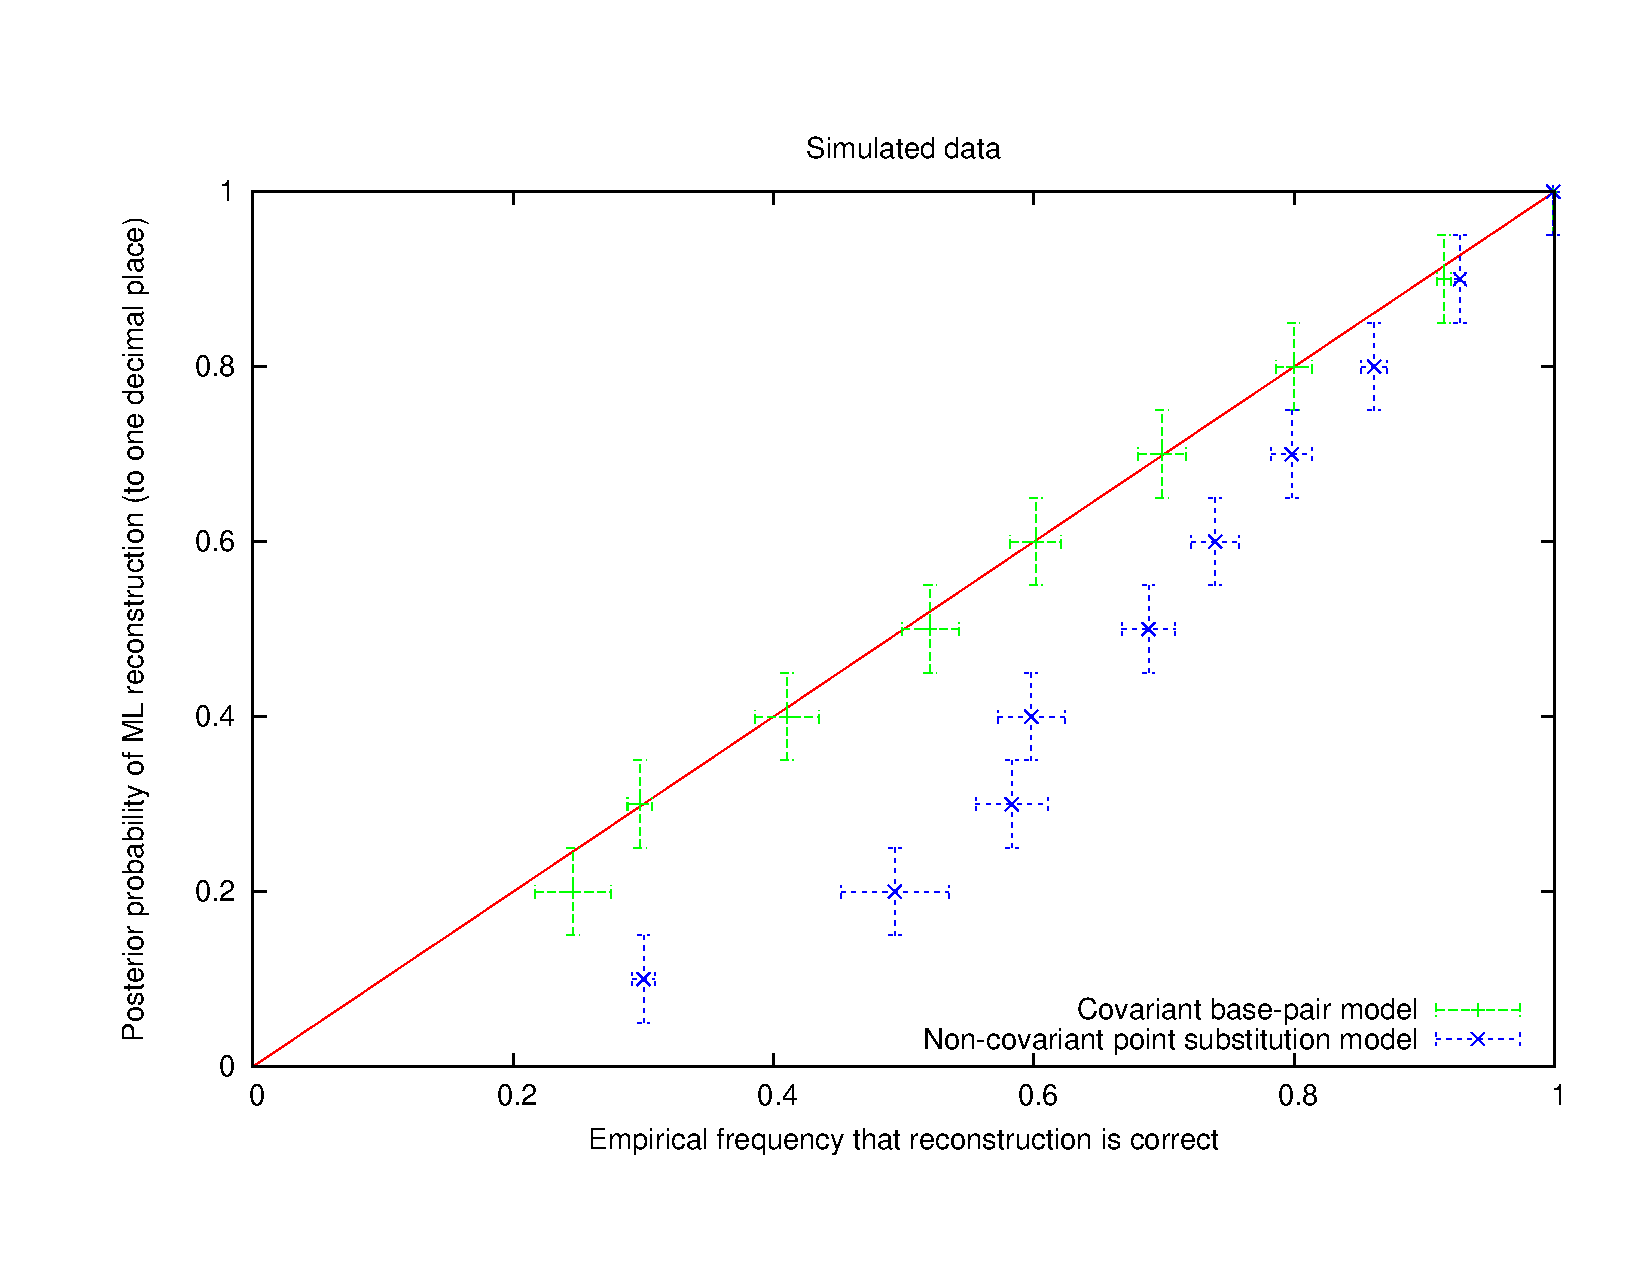
\includegraphics [width=0.45\textwidth] {figs/hammer_paired.pdf}
     \hspace*{\fill}
     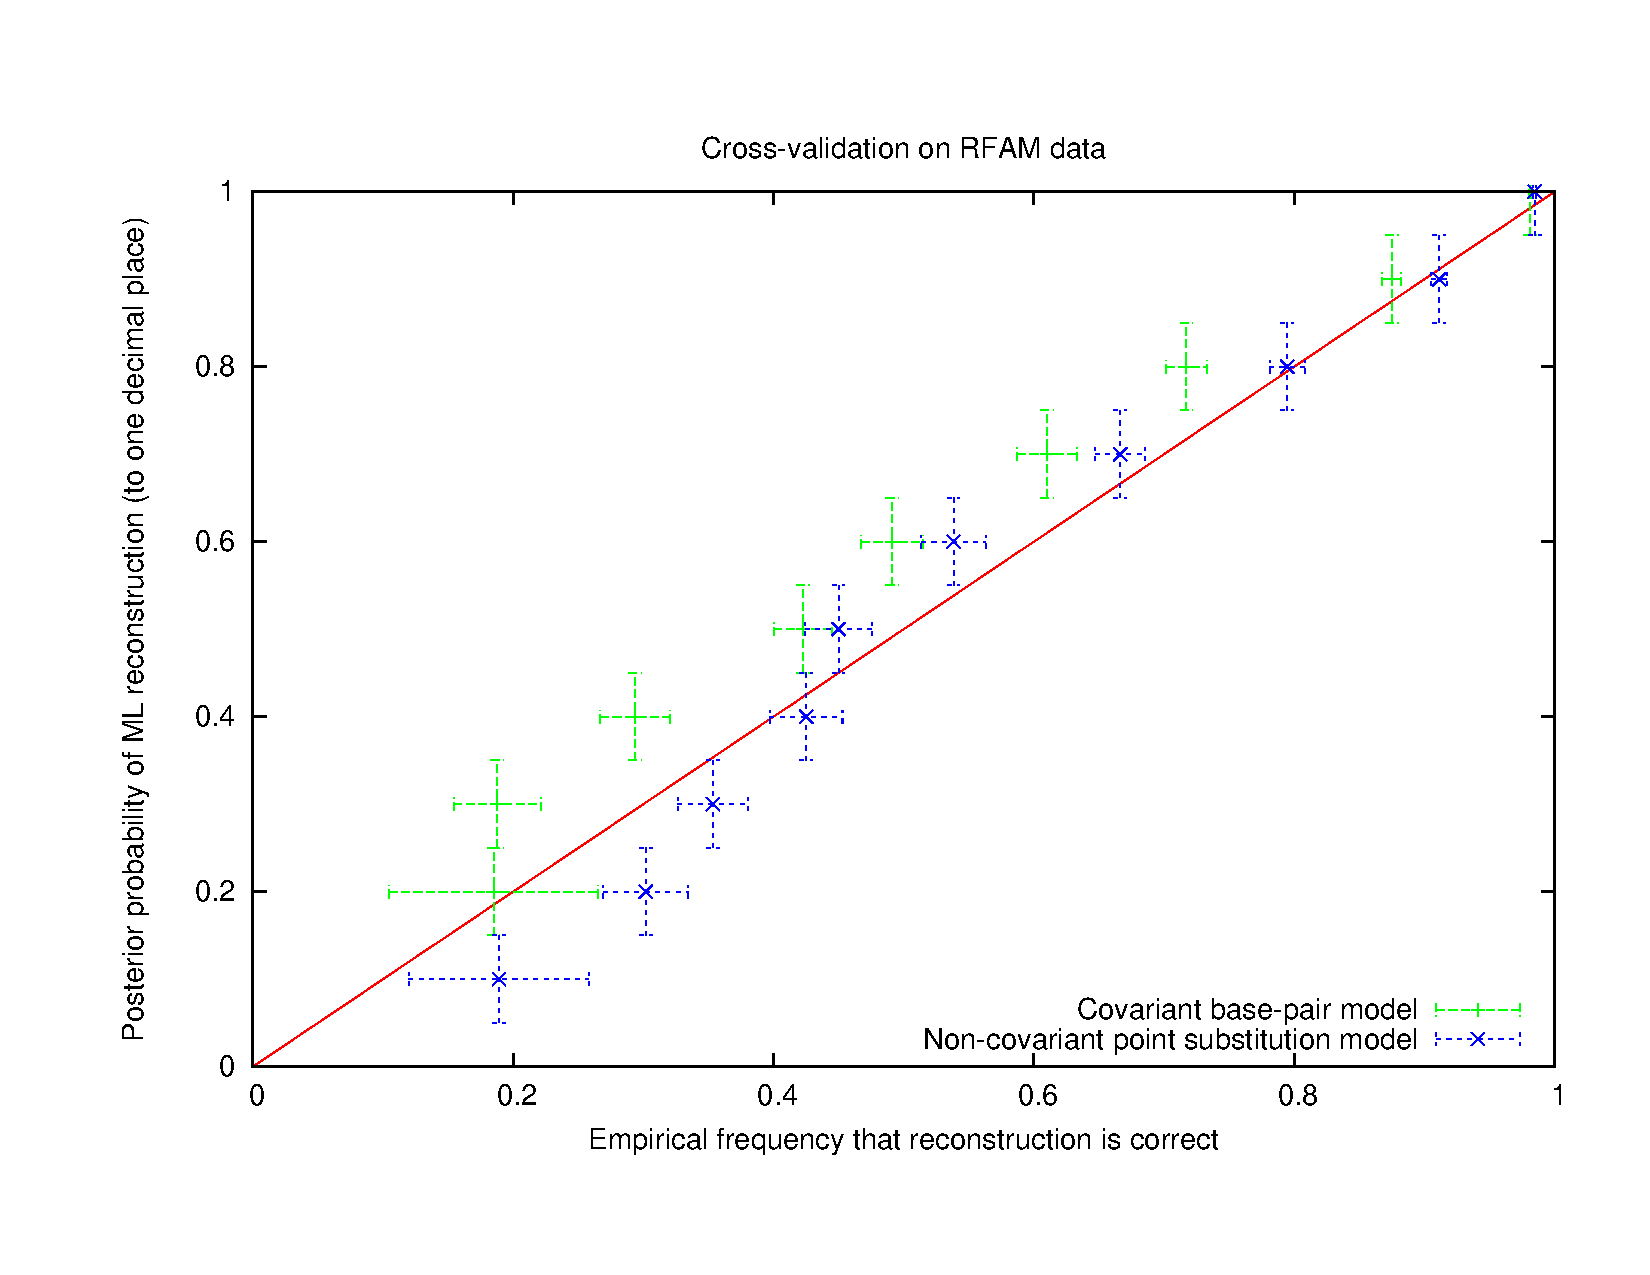
\includegraphics [width=0.45\textwidth] {figs/xval_paired.pdf}
  \end{center}
  \caption{
    \figlabel{simulation}
    Accuracy of confidence estimates for base-pair reconstruction in simulations (left) and cross-validations on real data (right).
    Reconstructions were performed using \xrate\ \cite{KlostermanEtAl2006},
    using both covariant base-pair substitution models
    and naive, non-covariant, single-base point-substitution models.
    The plots show the relationship between the posterior probability that a model-based base-pair reconstruction is correct (vertical axis),
    and the empirical probability that reconstructions with that posterior probability are actually correct (horizontal axis).
    If the model's posterior probability estimates are correct, these points should lie on a straight diagonal line.
    Left: simulation test on the hammerhead ribozyme phylogeny.
    A covariant model (estimated from rRNA alignments) was used to generate the simulated alignments on the given phylogeny; the same model was then used to reconstruct ancestral sequence and obtain confidence estimates.
    As expected, the model accurately estimates the probability that the reconstructed base-pair is correct.
    A naive, non-covariant model (the general reversible model, estimated from the same alignments) was also used for reconstruction and confidence estimates.
    This model {\em under}-estimates the probability of correct reconstructions,
    since its equilibrium frequency has a higher entropy than the covariant model:
    i.e. it assigns probability more evenly across the sixteen possible base-pairs (as opposed to the covariant model, which strongly favors the six canonical base-pairs).
    Right: cross-validation (``hold-one-out'') test using \RFAM\ alignments with published (verified) structures.
    Here, the covariant model slightly {\em over}-estimates the probability of correctness.
    The rRNA alignments (from which the model rates were estimated) have fewer non-canonical base-pairs than the \RFAM\ alignments,
    so that the covariant model entropy is slightly {\em lower} than the empirical base-pair distribution;
    this may explain the discrepancy.
    The naive model's confidence estimates are correct
    for high-accuracy reconstructions,
    over-estimates for medium-accuracy reconstructions,
    and under-estimates for low-accuracy reconstructions.
  }
\end{figure}

\figref{simulation} (left) shows the results of these comparisons.
When using the same (covariant) model for simulation and reconstruction, the posterior probabilities are an excellent unbiased estimate of the frequency with which the model reconstructions are correct.
However, the naive point-substitution model, which does not include covariant substitutions at base-paired sites, systematically under-estimates these probabilities.
% perl -e '$f=shift;for$m(qw(g n)){print "$m: ",100 * `grep "$m= 0" $f | wc -l` / `wc -l $f`,"\n"}' Hammerhead_1.bptest
In our simulation, the ancestral error rate for the naive model (4.9\%) was significantly higher than that of the covariant model (1.7\%).
% perl -e '$f=shift;for$m(qw(g n)){print "$m: ",100 * `grep "$m= 0" $f | grep "${m}can= 0" | wc -l` / `grep "$m= 0" $f | wc -l`,"\n"}' Hammerhead_1.bptest
Furthermore, 74\% of incorrect base-pairs predicted by the naive model were non-canonical (i.e. not AU, CG, GC, UA, GU or UG),
compared to only 2\% of incorrect predictions by the covariant model.

\begin{figure}[p]
  \begin{center}
     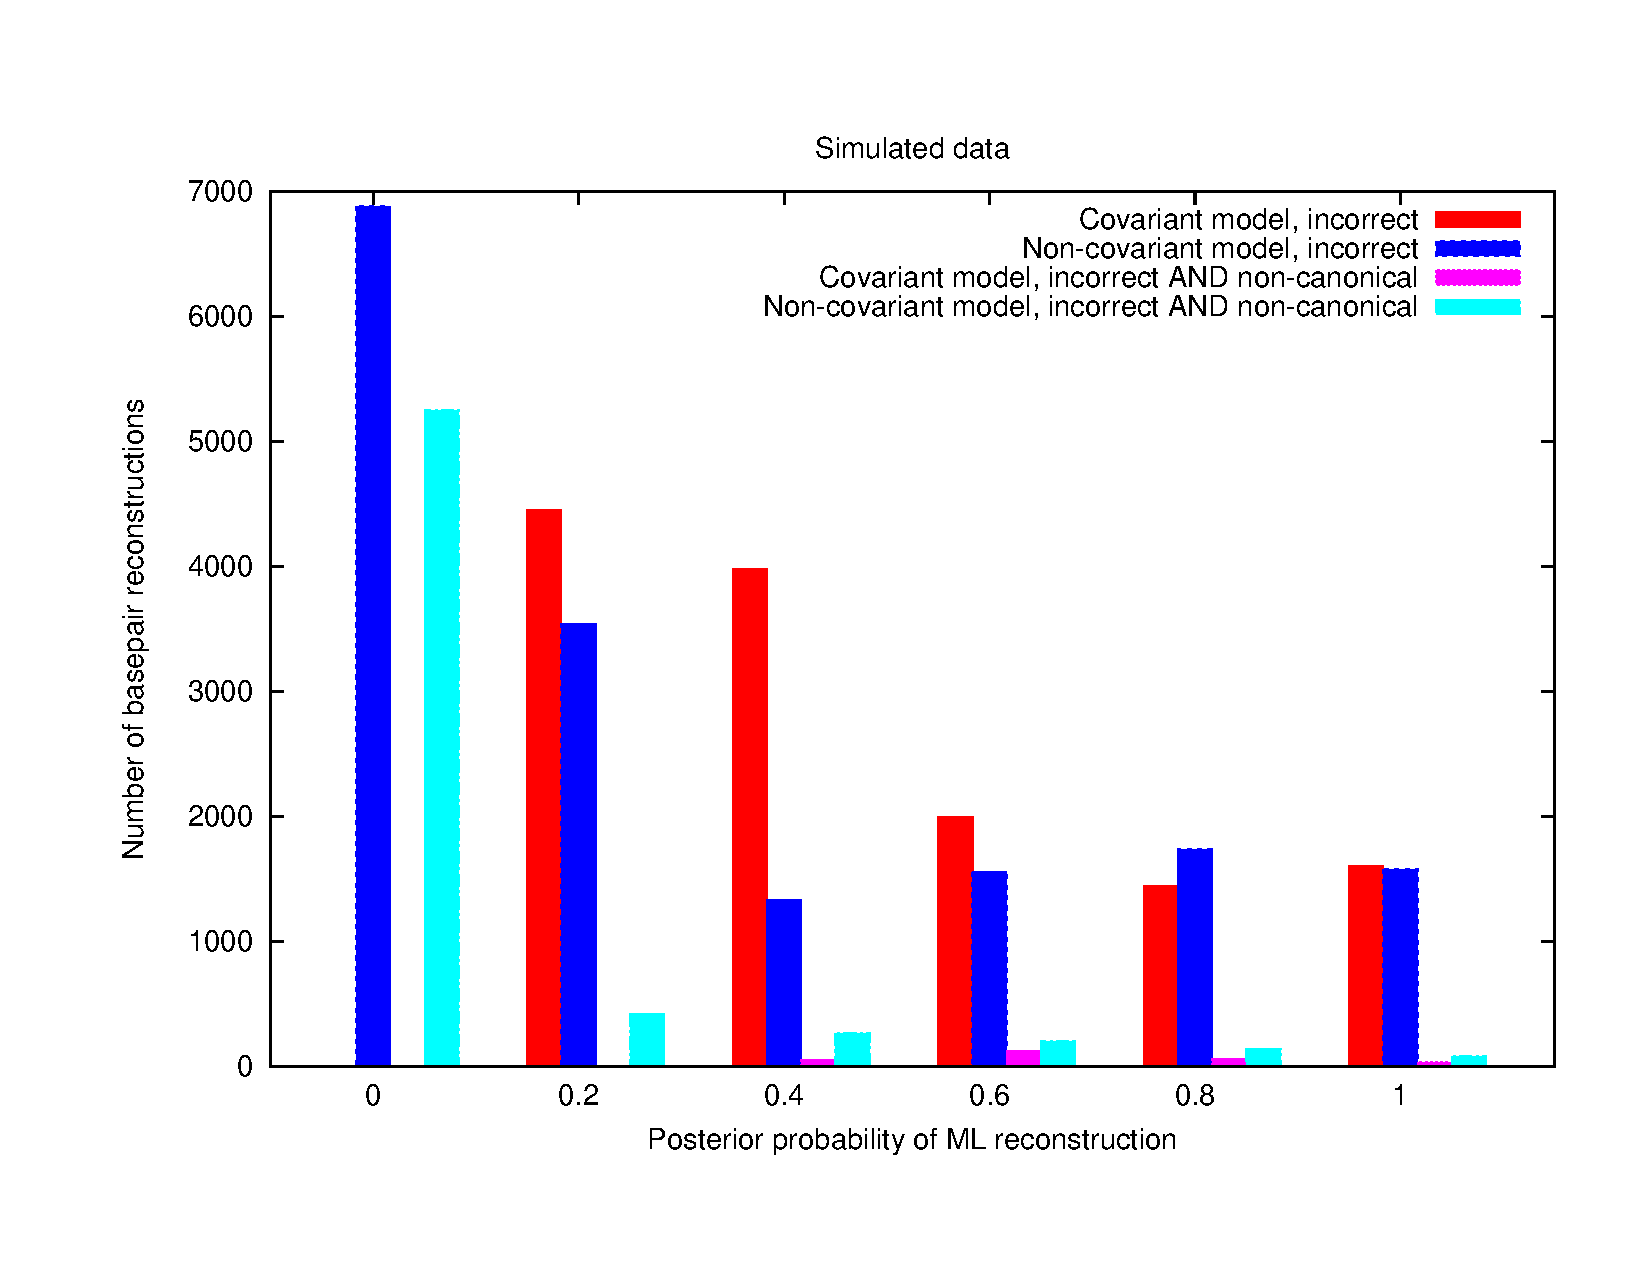
\includegraphics [width=0.45\textwidth] {figs/hammer_hist.pdf}
     \hspace*{\fill}
     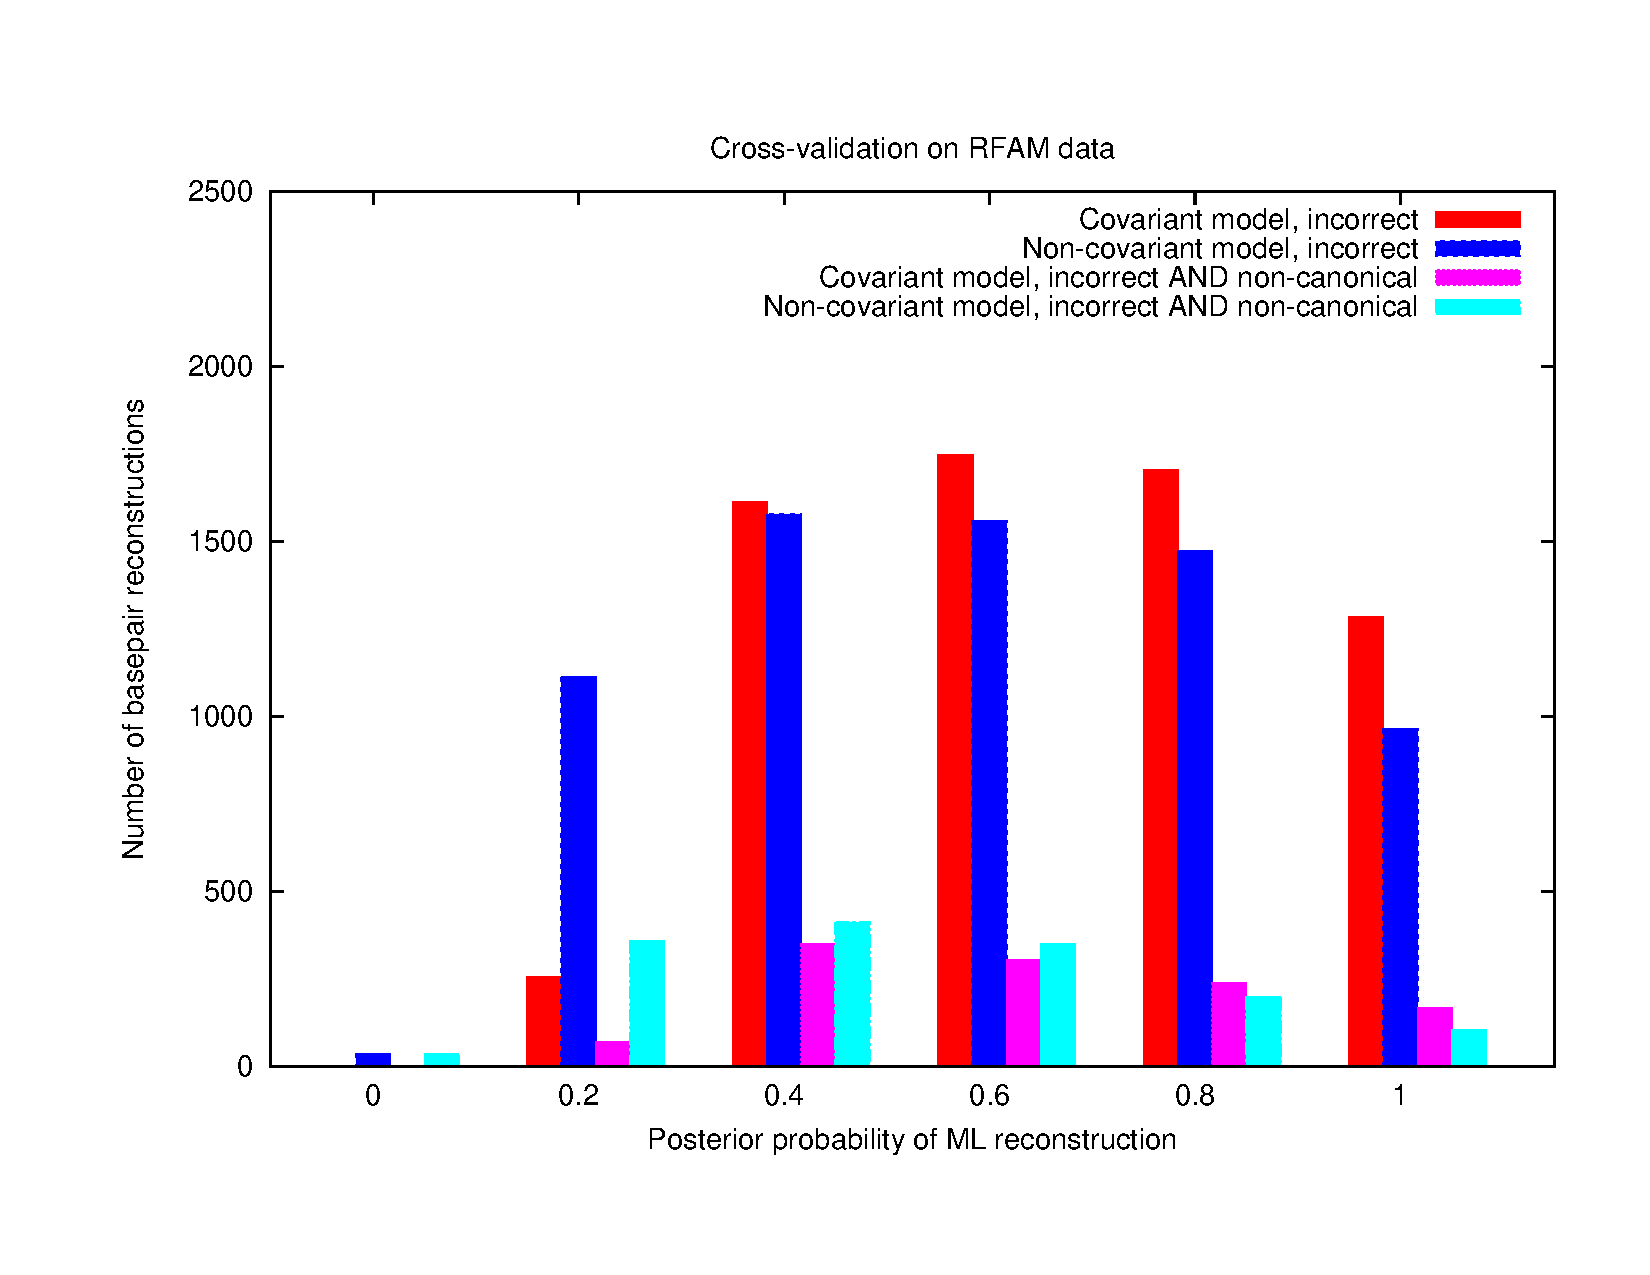
\includegraphics [width=0.45\textwidth] {figs/xval_hist.pdf}
  \end{center}
  \caption{
    \figlabel{histograms}
    Proportions of reconstructed base-pairs that are incorrect (and the subset of those that are non-canonical)
    in simulations (left) and cross-validations on real data (right).
    Base-pair reconstructions that are incorrect AND non-canonical
    might potentially disrupt a synthetic reconstructed structure.
    While the covariant model does not always get more base-pairs correct than the naive model,
    it predicts fewer non-canonical base-pairs.
    The sharpest difference between the models are in the lowest posterior-probability categories,
    corresponding to low-confidence predictions (e.g. sequences on deep branches, or base-pairs with few homologues).
    In this category, the covariant model also makes far fewer errors than the naive model.
    See main text and caption to \figref{simulation} for details of simulation and cross-validation procedures.
    \RFAM\ families with verified structures tended to be less phylogenetically diverse,
    with roughly half the total branch length (on average), than the tree used for our simulations;
    this may explain the relative paucity of low posterior-probability errors in the right-hand plot, compared to the left.
% perl -e 'use Newick;use Stockholm::Database;$db=Stockholm::Database->from_file(shift);for$a(@$db){next if$a->columns>500 || @{$a->seqname}>400;$tree=Newick->from_string(@{$a->gf_NH});$b=0;for$l(@{$tree->branch_length}){$b+=$l}print"$b\n"}' ~/rfam/Training/Published.stock | meansd.pl
% perl -e 'use Newick;use Stockholm::Database;$db=Stockholm::Database->from_file(shift);for$a(@$db){$tree=Newick->from_string(@{$a->gf_NH});$b=0;for$l(@{$tree->branch_length}){$b+=$l}print"$b\n"}' ~/rfam/Training/Hammerhead_1.stock
  }
\end{figure}

We also performed cross-validation (hold-one-out) experiments. Starting from \RFAM\ alignments whose secondary structure is labeled ``Published'' (i.e. experimentally validated),
we estimated phylogenetic trees using the neighbor-joining algorithm
with the Jukes-Cantor model,
then removed individual sequences
 and attempted to reconstruct them using \xrate.
(This is possible because the substitution models are time-reversible, so we can treat any node as ancestral.)
In this experiment, the error rates for base-pair reconstructions again differed by a few percent, though both error rates were higher than in the simulation test
% perl -e '$f=shift;for$m(qw(g n)){print "$m: ",100 * `grep "$m= 0" $f | wc -l` / `wc -l $f`,"\n"}' Published.xval-bptest
(covariant model: 11\%, non-covariant model: 16\%).
% perl -e '$f=shift;for$m(qw(g n)){print "$m: ",100 * `grep "$m= 0" $f | grep "${m}can= 0" | wc -l` / `grep "$m= 0" $f | wc -l`,"\n"}' Published.xval-bptest
Of the incorrectly-reconstructed base-pairs, the non-covariant model again predicted more non-canonical pairs (40\%) than the covariant model (17\%),
especially at lower confidence levels (\figref{histograms}, right).

Posterior probability estimates for both models were
systematically higher in the cross-validation test than they were in the simulation (\figref{simulation}, right).
The presence of this trend in both models
suggests that it may be due to differences between the European rRNA alignments
(from which the rates were estimated)
and the \RFAM\ alignments (which were used in the cross-validation test).
This is confirmed by our empirical observations of
covariant rate matrices estimated from the two alignment datasets:
base-pairs in the \RFAM\ alignments are more frequently
non-canonical, and appear to evolve faster (relative to single-stranded regions),
than base-pairs in the rRNA alignments
(for details, see {\tt biowiki.org/RnaModels}).
Repeating the cross-validation experiment with rates estimated from the \RFAM\ alignments,
we find the covariant model predicted slightly fewer non-canonical base-pairs
% perl -e '$f=shift;for$m(qw(g n)){print "$m: ",100 * `grep "$m= 0" $f | grep "${m}can= 0" | wc -l` / `grep "$m= 0" $f | wc -l`,"\n"}' Published.pubxval-bptest
(14\% rather than 17\%)
and produced slightly more accurate posterior probability estimates (data not shown).
Although this is no longer a strict cross-validation (since parameters were estimated from the test dataset),
it nevertheless emphasizes the value of correct models.
%Another possible source of errors in the cross-validation (compared to the simulation)
%is inaccurately estimated phylogenetic topologies and branch lengths;
%this might be improvable by using a covariant model in the phylogenetic estimation step (rather than Jukes-Cantor),
%and/or by using Bayesian phylogenetic estimation tools (rather than neighbor-joining).

Accurate estimates of posterior probabilities are likely to be important:
sub-optimal predictions are a significant piece of the reconstruction puzzle \cite{WilliamsEtAl2006,PollockChang2007,ChangEtAl2007}.
Ancestral reconstruction by probabilistic modeling does not yield a single definitive sequence, but rather a probability distribution over sequences.
Combinatorial synthesis by degenerate primer assembly has been advocated as a means of sampling from this distribution \cite{Gaucher2007}.
Nucleotide-perfect reconstructions may not always be possible:
it may be more productive to aim for accurate confidence estimates
(including sub-optimal predictions)
than to focus exclusively on getting everything right the first time.

Based on these tests, we conclude that deep phylogenetic reconstructions of ribosomes, and other RNAs, will require covariant substitution models that take account of RNA secondary structure.
We may reasonably deduce that indel reconstructions will, similarly, need to take account of RNA structure.
These results, therefore, strongly motivate the development of multi-sequence models for RNA structure, such as the TKF Structure Tree.



\section{Terminological asides}

This subsection contains some asides about terminology,
and can be omitted on a first reading of this paper.
The intent of this subsection is to highlight connections to related fields
in molecular evolution and computer science.

\subsection{Phylogenetic grammars}

We here describe some relationships to grammar models in current use in molecular evolution.

% Removing this sentence since I do not think that describing the relationship between transducers and SCFGs as an "injective mapping" will make it any clearer for most readers -- it is a bit like describing a string as a "concatenative monoid" -- IH
%There exists an injective mapping from the evolutionary models generated by our model-construction algorithm to multi-sequence SCFGs. In other words, 
Given a singlet transducer, a phylogenetic tree, and a mapping from tree to branch transducers,
the transducer composition algorithm returns a corresponding multi-sequence SCFG
which models the joint probability distribution $P(X_1 , ... , X_{n+m})$.

Several related bioinformatics grammars can be represented within this multi-SCFG framework,
allowing for substantial re-use of prior modeling theory:
\begin{itemize}
\item String transducers (which are similar to HMMs) can be viewed as special cases of parse-tree transducers,
without the facility to model long-distance correlations (base-pairs) or bifurcated structures.
\item Phylo-HMMs and phylo-SCFGs \cite{KlostermanEtAl2006}
can be viewed as special cases of (respectively) string transducers and parse-tree transducers.
(Phylo-HMMs and phylo-SCFGs typically model substitutions but not indels,
and so can be viewed as compositions of a richly-featured singleton transducer with a restricted class of branch transducers.)
\item Sakakibara \cite{Sakakibara2003} has described ``Pair HMMs on tree structures'' that are closely related to our parse-tree transducers
(though without the composition algorithms for scoring multiple alignments).
\item Sakakibara has also described pair stochastic tree-adjoining grammars, or TAGs \cite{Sakakibara2004}.
TAGs are a formal generalization of SCFGs to
mildly context-sensitive grammars \cite{MamitsukaAbe94,JoshiSchabes97,RivasEddy2000}.
We speculate that the conditionally-normalized transducer analogues of such Pair-TAGs may encompass the
phylogenetic model of covariant RNA substitutions and indels on pseudoknotted structures
described by \cite{MeyerMiklos2007},
just as parse-tree transducers encompass phylo-SCFGs.
\end{itemize}

\subsection{Statistical Alignment}

The term {\bf Statistical Alignment} was introduced by Hein \cite{HeinEtal2000}
to describe DP algorithms for phylogenetic grammars.
Although this term has been adopted by others in molecular evolution \cite{Miklos2002,Metzler2003,DrummondRambaut2007,SatijaEtAl2008},
we've avoided it (except in this section) for the following four reasons:
(i) Several RNA alignment methods already use another probability distribution
that's completely different to (though equally as valid as) the phylogenetic probability distribution over alignments:
namely, the Boltzmann probability distribution over secondary structures
\cite{GorodkinEtAl97,MathewsTurner02,HofackerEtAl2004}.
(ii) Many alignment tools make use of prior and posterior distributions over pairwise alignments
\cite{Miyazawa94,BucherHofmann96,Holmes98,BrayPachter2004,DoEtAl2004,Holmes2005,LoytynojaGoldman2005,SchwartzPachter2007,BradleyPachterHolmes2008};
all of these are arguably ``statistical'' alignment tools as well.
(iii) Some of the above-cited methods use sum-over-pairs alignment metrics, taking the expectation of such metrics over pairwise alignment posteriors,
and finding the multiple alignment that maximizes this expectation \cite{DoEtAl2004,SchwartzPachter2007,BradleyPachterHolmes2008};
others do progressive multiple alignment using pair grammars \cite{BrayPachter2004,Holmes2005,LoytynojaGoldman2005}.
Speculatively, such pair-based heuristics may (in some sense) approximate probabilistic alignment inference with true phylogenetic likelihoods;
similar convergences have, at least, been demonstrated between other pair-based heuristics \cite{EickmeyerEtAl2008}.
Thus, even using Hein's strict definition,
it's possible that a broad range of methods systematically {\em approximate} ``Statistical Alignment'';
this cautions against using the term too exclusively.
(iv) Even more broadly, many alignment tools make use of statistics to estimate alignment ``significance''.
In this frequentist approach, probability distributions for alignment scores (particularly Gumbel distributions)
are estimated for random sequences.
The tail integrals of these distributions then yield P-values for high-scoring database search results
\cite{KarlinAltschul93,Mott2000,Eddy2008}.
Thus, while the term ``Statistical Alignment'' has a quite specific technical meaning in molecular evolution
(a meaning which certainly encompasses the algorithms we describe here),
the broader bioinformatics literature may have competing claims to the term.
In any case, the goal of this work is statistical {\em reconstruction} of RNA protosequences,
rather than alignment {\em per se}.

\subsection{Parse trees and stacks}

Grammars are abstract models for languages;
finite-state automata are the corresponding abstract models for those languages' parsers.
Most of this paper uses the grammatical view of RNA structure evolution;
in this short section we digress briefly to mention the automata-theoretic view of these models.

The two non-local features that set SCFGs apart from HMMs are bifurcations and paired emissions \cite{Durbin98}.
In RNA structure analysis, these features are used to model (respectively) branched-loops and base-pairs.

A stochastic pushdown automaton can also model these features.
Such an automaton is essentially an HMM with a LIFO stack (LIFO = ``Last In, First Out'').

The pushdown automaton can parse two sequences simultaneously, aligning them and their parse trees.
It handles bifurcations and paired emissions by pushing symbols onto its stack:
a bifurcation by pushing a nonterminal, and a paired emission by pushing a terminal.
The pushed terminals and nonterminals are popped off the stack when the machine reaches its $\Send$ state.

The conditionally-normalized version of a pushdown automaton is a pushdown transducer:
a machine that absorbs {\em and} parses an input sequence (or absorbs an already-parsed input sequence)
and emits a (parsed) output sequence.
This is the machine that we describe as a parse-tree transducer.



\bibliography{../latex-inputs/alignment,../latex-inputs/duplication,../latex-inputs/genomics,../latex-inputs/ncrna}


\end{document}
